\chapter{Review of Cystic Fibrosis and The Molecular Basis of its Treatment}
\label{chap:cftr}
\chapquote{Because of what's inside me; Because of my genes.}{-Bob Flanagan ``Why?" \cite{dick1997}.}
\newpage
%Authors note:
% We begin with a breif overview of the disease Cystic Fibrosis as it is the main motiation for this project. A horrendous disease for which we will hopefully soon find a cure.

%Clinical outcomes are a chronic illness which affects multiple organ systems and every aspect of a patient's life. 
	%physical therapy, pancreatic sufficiency, ongoing discovery of chronic issues. Much to do. 


% The cause of the disease is CFTR misfunction.
       % CFTR function overview

% CFTR modulators act to restore its function. 
	% patients with rare genotypes cant access modulators.

We aim to elucidate the molecular nature of Cystic Fibrosis (CF)--A disease caused by the misfunction of a protein called the Cystic Fibrosis Transmembrane conductance Regulator (CFTR). In subsequent chapters we will use Molecular Dynamics (MD) to determine how rare mutations cause cause this protein to misfunction. These results are presented with the goal of building a molecular understanding for the treatment of rare CF causing mutations. Given the importance of the CFTR protein system to this work, we will look at its structure and dynamics in some detail in this chapter. In some sections of this chapter I have gone into far more detail than necessary in order to compile details which might serve as a reference text for future endeavours into molecular studies of CFTR. 

To understand the motivation for this level of detail, we will first review some of the medical literature surrounding the disease itself. CF is a multi-system disease with many complications. The management of symptoms can be a significant burden for patients and their families but recent treatments and advancements in translating basic biological research into the clinic has given many hope of a more normal life. 

After this review of clinical outcomes, we will once more work our way upward, as ultimately, CF symptoms are due to the mutation of a single gene. The detailed outline of CFTR structure and function will be our starting point for a physical understanding of CF pathogenesis. This will then be followed by an overview of the mechanism behind the restoration of CFTR by small molecule drugs known as CFTR modulators. 

Here we will also show how to integrate our molecular perspective from simulations with \textit {ex vivo} organoid models grown from a patient's own cells. Results from these organoid models will be presented in subsequent chapters to prove that small molecule drugs appear to be capable of treating a diverse set of molecular phenotypes. In chapter \ref{chap:conclusion} we will combine these results to argue that this personalised approach to medicine leads us to expect that patients with rare missense mutations will likely benefit from existing treatments, but they are currently excluded from accessing due to an outdated understanding of disease pathogenesis. 

The end of this chapter will contain a brief overview of the different experimental techniques which were employed by collaborators of our simulation work to characterise the response of different mutations to different drugs. The language in these sections is kept simple, so the unfamiliar physicist reader can understand some common techniques which they will encounter in the literature surrounding biochemistry and cell biology. The intention here is not replication but comprehension. Hence, an experienced biochemist or a cell biologist would likely find these explanations lacking. For a deeper understanding, the physicist is encouraged to spend lots of time learning from their experimental colleagues, or even perform some of these experiments themselves if possible. 

Another small deviation of this chapter compared to the previous chapters is the chosen structure. In previous chapters we always began with the smallest physically relevant length scale and then worked upward. In chapter \ref{chap:methods} I showed how we can begin from Schr\"odinger's wave equation and work to build simulation techniques which let us understand whole biomolecular systems. This was to give an example of the philosophy outlined in chapter \ref{chap:introduction}, where the physicist designs abstract formalisms and integrates them to model macroscopic physical phenomenon. In this chapter I have made a small but concious deviation from this pattern. Instead of beginning with a discussion of the smallest physically relevant system, the protein which causes disease, we will first discuss some of the clinical realities of living with CF. This deviation from a purely physics inspired structure is made so that we do not lose sight of our goals when studying biophysics.

When one trains to practice medicine they are taught how to conduct themselves ethically, with their patients best interests at heart \cite{hajar2017}. Typically, a physicist has no such training, so they may miss the human aspect of medicine by studying disease impersonally \cite{foucault1994}. 

In subsequent chapters we will work with the theoretical and impersonal tools of molecular physics, to understand the cause and treatment of a disease. We do this in the hope that a physical understanding may improve patients' lives. However, when using such techniques we must always remain aware of how such technologies could be misused in living systems. Consequences of the callous pursuit technological advancement can be seen in the participation of physicists in political and moral discourse in the 20th century. Here, the contributions from physicists were varied and not always for the better \cite{frank1993, gottfried1999, global2009, rhodes1986, aaronson2008, berger2016, vonneumann_britanica}. Should we wish to embark on the enterprise of studying biophysics we have a responsibility to do so ethically. Thankfully, many important questions have been studied by philosophers, and the reader is encouraged to seek texts on bioethics and also ethics in the use of artificial intelligence \cite{buchanan2000, taneri2011, genome_editting_guildelines_2017, muller2021, bostrom2014, roose2022}. These considerations are likely to become increasingly important---as biophysics advances, so too does its capacity for misuse \cite{mallapaty2022, urbina2022}. 

%The reader is asked to keep this responsibility in mind in the subsequent chapters where we have worked with basic, impersonal theoretical tools in molecular physics. These techniques were understand the cause and treatment of Cystic Fibrosis. This work was performed in the hope  do this in the hope that an increased understanding may may improve patients' lives. We must be aware of the moral pitfalls that a single minded pursuit of a physical understanding of living systems presents. We must be aware moral challenges that this represents. In the 20th century, physicists often participated in political and moral discourse, and not always for the better \cite{frank1993, gottfried1999, global2009, rhodes1986, aaronson2008, berger2016, vonneumann_britanica}. Should we wish to embark on the enterprise of studying biophysics we have a responsibility to also study how to do it ethically. Thankfully, many important questions have been studied by philosophers, so the reader is encouraged to seek texts on bioethics and also ethics in the use of artificial intelligence \cite{buchanan2000, taneri2011, genome_editting_guildelines_2017, muller2021, bostrom2014}. These considerations are likely to become increasingly important---as biophysics advances, so too does its capacity for misuse \cite{mallapaty2022, urbina2022}. 


%On this somewhat somber note, we will now take a brief look at what it is like to live with Cystic Fibrosis.

%We will then analyse the root cause, mutations to the Cystic Fibrosis transmembrane Conductance Regulator (CFTR). In chapter \ref{chap:conclusion} we will use much of the knowledge gained in this chapter to think about where we can direct future studies to help treat the root cause of Cystic Fibrosis. 

\section{Clinical Realities of Living with Cystic Fibrosis}
\label{clinical_realities_CF}
Cystic Fibrosis (CF) is the most common fatal genetic condition in Caucasian populations. Over 162 000 people are estimated to be afflicted globally, with a significant proportion living undiagnosed \cite{hammoudeh2021,guo2022}. Even with decades of research there is no known cure for CF and patients currently have a life expectancy below 50 \cite{mcbennett2022}. Management of disease symptoms also bears significant financial and emotional costs to patients and their families \cite{vangool2013, page2022}. From a cellular perspective, the symptoms of the disease are due to the inability of certain cells to regulate their salt content, causing an osmotic imbalance (Figure \ref{CF_summary}) \cite{reddy2013}. 

\begin{figure}
	\label{CF_summary}
	\begin{center}
	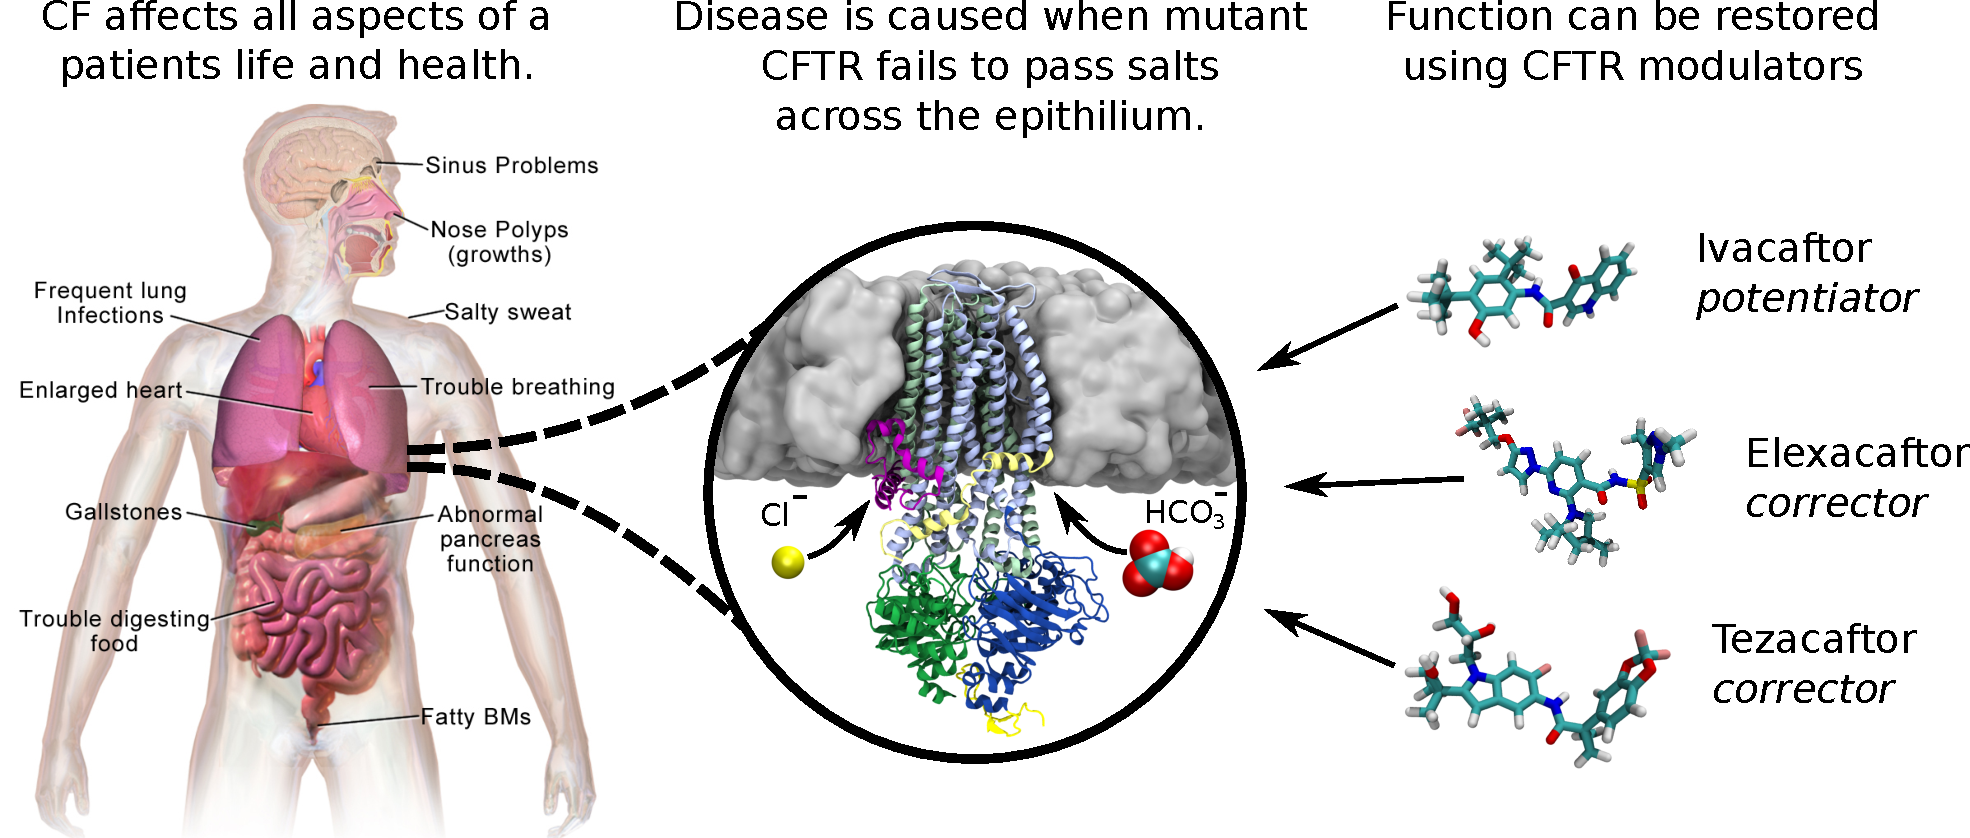
\includegraphics[width=1\textwidth]{figures/cf_summary_fig.pdf}
	\end{center}
	\captionsetup{singlelinecheck = false, justification=raggedright}
	\caption[Cystic Fibrosis is a Debilitating Disease Whose Cause is Genetic] {\textbf{Cystic Fibrosis is a Debilitating Disease Whose Cause is Genetic}}{Cystic Fibrosis causes misfunction in several major organ systems, affecting all aspects of a patients' life and health. The cause of the disease is genetic, when two defective copies of an anion channel gene, CFTR, are inherited from each parent, epithelial cells cannot pass chloride or bicarbonate ions, leading to a pathogenic buildup of salts inside epithelial cells. In recent decades, small molecule drugs have been discovered which act directly on CFTR to restore its function. This thesis seeks to understand what kind of defects these drugs are capable of rescuing. We find that they are likely to rescue a wide range of defects.} 
\end{figure}

All organs of the body are lined by cells called epithelia. They protect organs from trauma and infection. The most acute symptoms of CF are due to the dehydration of this lining. When dehydrated, fine, motile structures on the epithelium called cilia collapse, rendering them unable to ``beat" in order to clear mucus and pathogens \cite{boucher2007, szczesniak2017}. Simultaneously, this mucus which naturally lines the epithelium, thickens as moisture is leached away from it by osmotic pressure.

This thickened mucus has pathogenic effects in several organ systems. The most acute symptoms occur in the lungs where bacterial colonies grow and form a biofilm. This damages the organ and remains one of the most troublesome chronic complications for CF patients \cite{chiappini2014, krouse2001}. Frequent infections mean that patients rely on antibiotics and avoid other people with CF in case they expose each other to new or drug resistant pathogens \cite{conway2008, baldoni2019}. 

In addition to these bacterial colonies, the buildup of mucus inhibits the normal function of the lungs, limiting their ability to absorb oxygen. Patients often undergo hours of physical therapy each day to help them clear this mucus from their lungs \cite{chest_pt_CFF,thefreylife2015}. Inhalation of a saline solutions may also help relieve symptoms, as this draws moisture out of the epithelial cells by counteracting the pathogenic osmotic pressure gradient \cite{wark2018}. As Figure \ref{CF_life_expectancy} indicates, much of the increased life expectancy for people with CF has been due to the improved management of this mucus and the populations of bacterium infecting it \cite{mcbennett2022}. 

In CF care, maintaining lung function remains the primary concern. The organ gradually fails over the course of the patients life, meaning respiratory failure is usually the cause of death \cite{kumar2018}. The adoption of lung transplants has lead to a significant increase to the life expectancy of CF patients but patients may be excluded from receiving a transplant for a variety of reasons \cite{blatter2015, weill2018}. Double lung transplants remain the only option for CF patients as the donor lung would become infected with bacteria from the CF afflicted lung left in their body \cite{mcbennett2022}. 

To track disease progression, the most commonly used biomarker is FEV1\%. This stands for Forced Expiratory Volume in 1 second. It is a measure of the volume of air a patient is able to forcibly expel in one second, compared to their total lung capacity \cite{szczesniak2017}. Once a patient's FEV1\% falls below a certain level (30\%-50\%) they will usually begin to consider a lung transplant if they are eligible \cite{adler2009}.

CF also causes acute and chronic issues in the digestive system. Due to the buildup of mucus, the large intestines struggle to absorb nutrients and the pancreas cannot secrete digestive enzymes. These complications can lead to CF related diabetes which afflicts roughly half of adults with CF \cite{Kayani2018}. To manage and avoid this complication, patients are administered digestive enzymes and consume a high fat diet \cite{sullivan2017}. A patient whose pancreas does not produce sufficient enzymes to digest nutrients is referred to as ``pancreatic insufficient" (PI). This is an important determinant in the severity of disease and a patients' quality of life \cite{halloran2011,singh2017}. 

\begin{center}
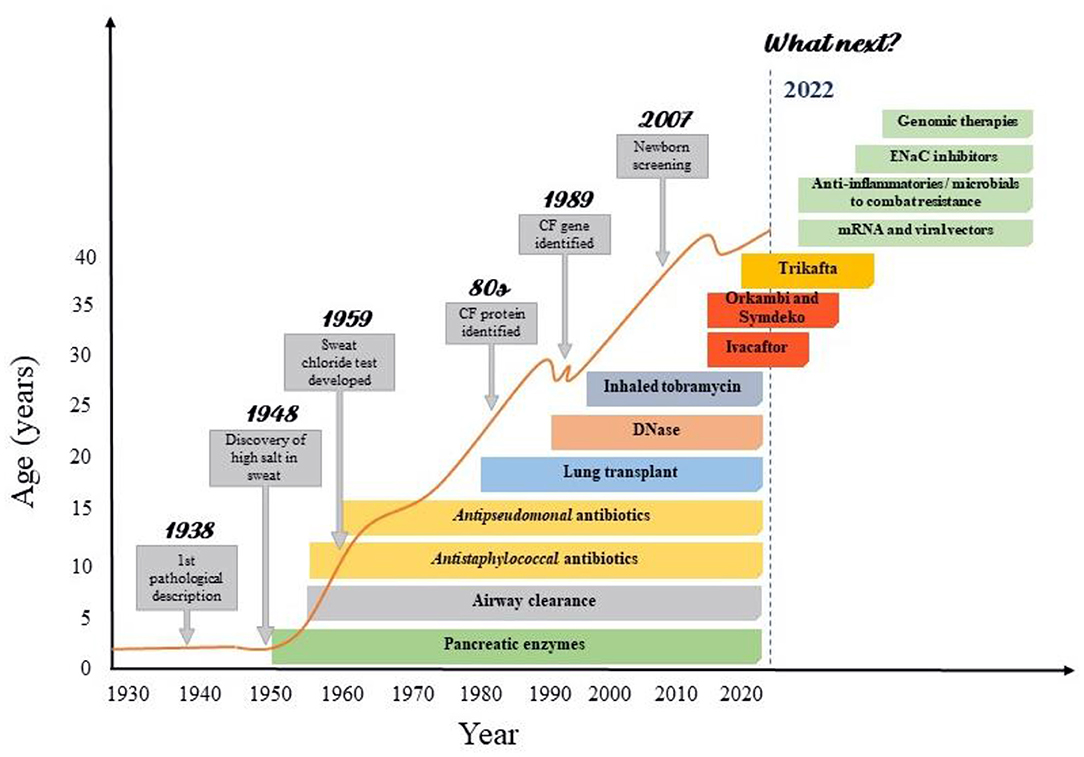
\includegraphics[width=0.7\textwidth]{figures/CF_life_expectancy.png}
\end{center}
%\captionsetup{singlelinecheck = false, justification=raggedright}
\begingroup
\captionof{figure}[CF Clinical Progress] {\textbf{CF Clinical Progress}}{The orange line depicts the life expectancy of CF patients in relation to the development of different treatment. Life expectancy correlates highly with translational research. As CF becomes a chronic condition patients will likely undergo a combination of more and more advanced therapies. Source \cite{garcia2022}} 
\label{CF_life_expectancy}
\endgroup

Figure \ref{CF_life_expectancy} displays something quite interesting. As patients live longer, CF care must address more disease complications. For example, once pancreatic enzymes were routinely administered, patients began to live beyond two years old \cite{roberts1957, levy2011}, which lead to an to an increasing need to study and manage the role of bacterial infections in the CF lung \cite{burns2001}. With the advent of modulators and refinements to existing therapies, the face of the disease will change. Now that patients are living past 40 we must confront new complications such as bone disorders and infertility \cite{stalvey2013, popli2007}. This means that there still a need to study the cellular and molecular nature of CF, both its root cause and the cause of complications. 


\section{The Misfunction of CFTR Causes Cystic Fibrosis}

We will now begin our journey upward. As we mentioned in the introduction, we will be collecting molecular details about the ion channel at the core of CF pathogenesis to understand the disease and its treatment. Hence, the next sections will outline in considerable detail, the structure, function and misfunction of the CFTR anion channel. 

CFTR is unique. It is a type of protein known as an ABC transporter, designated ABCC7. The ABC super family of proteins bind ATP and use the energy from hydrolysis (breaking) ATP to pump different substrates across the cell membrane, against a concentration gradient. But CFTR does not act as a transporter like the other members of its family. Rather, it can be thought of as a ``leaky pump" since it moves through through a gating cycle but is unable to move its substrate against against a concentration gradient \cite{gadsby2006,linsdell2018}. It is possible that the evolutionary misappropriation of this protein from a transporter into an ion channel is the reason for the large number of mutations which cause it to misfunction \cite{infield2021}. 

%Hence, as CFTR is an \textit {ion channel}, meaning it allows the passive diffusion of chloride and bicarbonate, but it can also pass larger anions such as glutathione (figure \ref{}) \cite{gadsby2006, tang2009,linsdell1998}. 

\subsection{CFTR structure and function}

\begin{figure}
	\begin{center}
	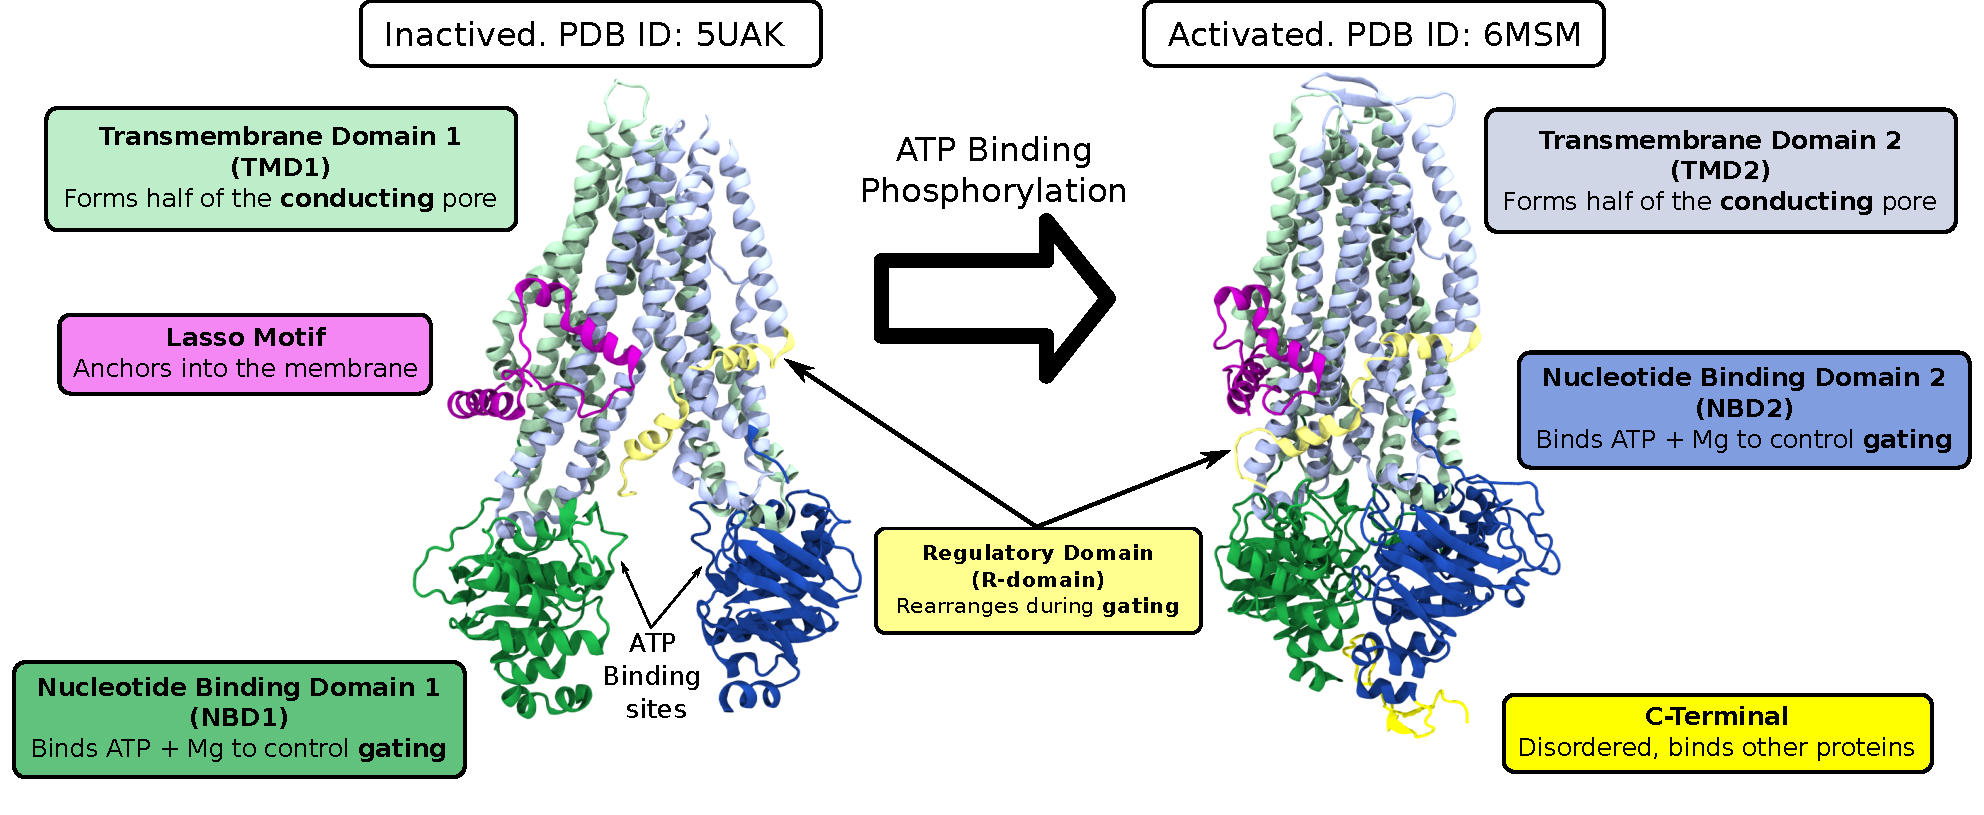
\includegraphics[width=\textwidth]{figures/CFTR_structure.pdf}
	\end{center}
	\label{CFTR_structure_domains}
	\captionsetup{singlelinecheck = false, justification=raggedright}
	\caption[CFTR Structure] {\textbf{CFTR Structure}}{There are currently two conformations of the human CFTR protein which have been imaged at atomic resolution. These cryo-EM structures have captured hCFTR in an inactivated and an activated conformation. The inactivated state (PDB ID: 5UAK) is neither phosphorylated nor bound to ATP. Observe how the NBDs are far apart and the TMDs are not parallel, forcing a constriction near the top of the protein which does not allow the passage of ions. By contrast, the activated structure is bound to two ATP molecules (PDB ID:6MSM), dimerizing the NBDs and bringing the TMDs into a parallel configuration where they are able to form a pore. Despite having the biochemical characteristics which we would expect from the conducting conformation of this ion channel, the available structure of the activated hCFTR protein exhibits a constriction at the extracellular end of the channel which does not allow chloride ions to pass through. In chapter \ref{chap:opening} we will demonstrate enhanced sampling techniques to study a fully conducting CFTR conformation, based on this activated structural snapshot. All simulations presented in this work were based on the ATP-bound phosphorylated human CFTR structure (PDB ID: 6MSM) \cite{zhang2018}.} 

\end{figure}

As an ATP stimulated ion channel, CFTR sits in an inverted ``V" configuration in the cell membrane until it is activated by chemical messengers like ATP and PKA \cite{zhang2018, gadsby2006, mihalyi2020}. When it is phosphorylated, the protein transitions to form a continuous pore. This is the conformational change visualised in Figure \ref{CFTR_structure_domains}.

Chemically speaking, the protein is composed of a single chain of 1480 amino acids.  This chain folds into a pseudo-symmetric structure, organising CFTR into 7 domains. In the order of their primary structure they are: 

\begin{enumerate}
	\item The Lasso motif (AA 1-68), Which anchors into the membrane and serves as an interaction hub with protein partners such as syntaxin and filamin which are important in cellular trafficking \cite{cormet-boyaka2002, naren1998, thelin2007}. 
	\item Transmembrane Domain 1 (TMD1, AA 69-376). This domain forms half of the chloride conducting pore and importantly, TM1 and TM6 in this domain form the extracellular end of the pore for anion permeation \cite{linsdell2006, linsdell2022}. Most positive amino acids which directly interact with anions are located in this domain, even in the inner vestibule \cite{linsdell2018}. We will look at many of these amino acids in detail in chapters \ref{chap:R352Q} and \ref{chap:opening} \cite{wong2022a}. There is a pocket in this domain which also serves as a binding site for both corrector class drugs and protein partners such as WNK1, which stimulates the conductance of bicarbonate \cite{kim2019}. 
	\item Nucleotide Binding Domain 1 (NBD1, AA 377-629). One of the ATP binding sites. This domain has a dense concentration of disease causing mutations, including the most common mutation $\Delta$F508 \cite{cftr2}. This domain contains a Walker A motif but lacks a Walker B motif. This causes one of the ATP binding sites to be degenerate meaning it cannot hydrolyze ATP. 
	\item Regulatory Domain (R-domain, AA 630-855). A disordered domain containing more than 11 phosphorylation sites \cite{mihalyi2020}. In the inactivated conformation of CFTR, a helical segment of this domain wedges between the TMDs. Binding to PKA encourages this helix to unwedge from between the TMDs, while phosphorylation causes the disordered domain to remain in solution. This process has important consequences for the function of the channel \cite{ostedgaard2000, mihalyi2020, bozoky2013, baker2007}. In the open state, the wedge relocates to a location just below the lasso motif \cite{zhang2018}. The identity of the wedge fragment will be analysed in detail in chapter \ref{chap:I37R} \cite{wong2022}. 
	\item Transmembrane Domain 2 (TMD2, AA 856-1168). This domain forms the other half of the chloride conducting pore. There is some controversy over the structure and function of TM8 in CFTR \cite{hegedus2022, liu2019}. This helix plays a critical role in regulating channel gating and anion selectivity \cite{negoda2019}.
	\item Nucleotide Binding Domain 2 (NBD2, AA 1169 - 1450). One of the ATP binding sites. This domain is home to a conserved Q-loop, which regulates the binding of ATP in ABC transporters \cite{ivey2020, zolnerciks2014, dong2015}. NBD2 contains both a Walker A and a Walker B motif, allowing ATP binding and hydrolysis at what is known as the consensus binding site. 
	\item C-terminus (AA 1451 - 1480). This domain is natively disordered but it serves as an interaction hub in WT-CFTR, anchoring CFTR to other proteins in the cell through its PDZ binding domain \cite{moyer1999, cushing2008}. 

\end{enumerate}


%CFTR is distinguished by a regulatory region known as the R-domain (residues 645-845) which links NBD1 to TMD2. This region acts to lock the channel in the closed state by wedging itself between the TMDs and dislodging when any one of 3 sites are phosphorylated \cite{mihalyi2020}. In experimentally determined structures of human CFTR the secondary structure of a section of the R-domain but not at high enough resolution to determine the identity of individual side chains \cite{zhang2018, zhang2016}. Further secondary structure information can be found through experiments with NMR \cite{Baker2007}.

\subsection {Previous MD Studies of CFTR}
Because the first structure of human CFTR was only published in 2017 \cite{liu2017}, previous computational studies of CFTR have had to rely on homology models. More recently these were based on the phosphorylated zebra fish protein ( PDB ID:5W81) \cite{zhang2017a} or for a longer time, a distantly related bacterial ABC transporter SAV1866 ( PDB ID:2HYD) \cite{dawson2006, Hoffmann2018}. These studies have yielded interesting results but it is often hard to translate their findings to the human protein. Even in the zebra fish CFTR protein, the similarity to the human amino acid sequence is only 55\%. This raises some concerns. As we will see, CFTR is a highly sensitive protein, its function is poorly conserved under mutations. Note for example how note is how the action of certain drugs is not conserved in zCFTR \cite{laselva2019}. Additionally, the short time scales (rarely reaching 500ns) of the simulations in these studies opens the possibility that the homology model of the protein remained trapped in local minima, raising questions as to the reliability of their findings.  

Despite their short comings the publications which employed these homology models to investigate the basic function of the CFTR protein have a few notable findings which we will discuss briefly. 

Perhaps the most interesting molecular study from this era used path-CV metadynamics to propose open state of the channel by steering a zebra fish based homology model toward fully outward facing conformation of SAV1866 \cite{Hoffmann2018}. The resulting model has several characteristics expected of the open channel, such as the critical R117-E1124 and R352-D993 salt bridges. However, it fails to create a narrow selectivity filter, which we would expect given results from \textit{in vitro} biophysical experiments \cite{linsdell2016, linsdell2017, linsdell2021, li2018b, linsdell2020, negoda2019}. Additionally, the free energy landscape in this study does not actually display a free energy well at the coordinates which the authors state corresponds to the open state, nor did they validate their open structure with long unbiased simulations (runs were truncated after 50ns). This raises some questions as to whether their proposed open conformation was indeed stable in their model system. However, it was the innovative use of metadynamics in this study which served as the inspiration for the extensive free energy calculations in chapter \ref{chap:opening}. Hence, it was this ambitious study which allowed us to discover a fully open conformation for the human channel. 

A more recent study again employed metadynamics with the zebrafish structure, to study the permeation of chloride through the two extracellular portals in zCFTR \cite{farkas2020}. Unfortunately, this confirmed a difference between the zebrafish and the human structures. Experimental studies indicate that only one extracellular portal is present in the human structure \cite{linsdell2018}. 

Another study, still under review at the time of writing, attempted to resolve the chloride permeation pathway in the same human, phosphorylated CFTR structure which we have investigated in this thesis \cite{zeng2021}. Here, Zhi Zheng, working under Reggis Pomm\'es used unbiased MD coupled with an induced 500mV membrane potential. This strong electric field was used to encourage chloride ions to move through the channel. This study was successful in observing 17 conduction events in 10$\mu$s of unbiased sampling. Although excellent progress, this is an order of magnitude below the number of conduction events we would expect from this level of sampling--given that the conductivity of the open conformation in WT-CFTR is 0.7pS \cite{kogan2003,linsdell1998}. These implications will be discussed in chapter \ref{chap:opening}.

There are some additional MD and docking studies which have either dealt with the effects of mutations or the action of CFTR modulators and they will be discussed in the relevant sections of this chapter (section \ref{} \ref{} respectively )\cite{billet2020, sabusap2021}.

In terms of the basic investigation into the function of CFTR, the final study we will discuss simulated of both human and zebra fish structures were used to study the conformation of TM8 in TMD2 \cite{corradi2018}. As we will discuss in detail in chapter, \ref{chap:conclusion} all CFTR structures solved by the Chen lab exhibit an unusual fold in TM8 \cite{fiedorczuk2021, liu2017, liu2019, zhang2016, zhang2018a, zhang2017a}. The helix unwinds in the middle of the membrane, a configuration that was initially thought to be energetically unfavourable. At the time of writing, there are some unresolved questions as to how this conformation is consistent with low resolution structures of chicken CFTR solved by another laboratory \cite{fay2018}. However, most recent studies have supported the TM8 model found by the Chen lab \cite{corradi2018, negoda2019}. 

In summary, with some exceptions, it is difficult to draw from the previous \textit{in silico} literature of CFTR because studies have lacked an appropriate structure as a starting point. Previous CFTR homology models have largely failed to capture critical molecular details of the full human CFTR protein. Hence these studies mostly served as a proof of concept and inspiration for further work, rather than giving results which can be directly inferred for the hCFTR protein. 

% , it lacks a salt bridge between R104-E116. In experiments, these residues could be replaced by cysteines and the channel would still function. However, when reducing agents were added to the system the channel lost its ability to open fully. This indicates that in the oxidised environment the C104-C116 cysteines formed a disulfide bridge but its breaking upon exposure to reducing agents caused a loss of function in the channel. This indicates that in the WT channel R104-E116 form a stable salt bridge. 

%This salt bridge is clearly visible in the recent cryo-EM structure of ATP-bound human CFTR \cite{zhang2018}.

\subsection{Catalytic and Conformational Changes During the Gating Cycle}

	\begin{center}
	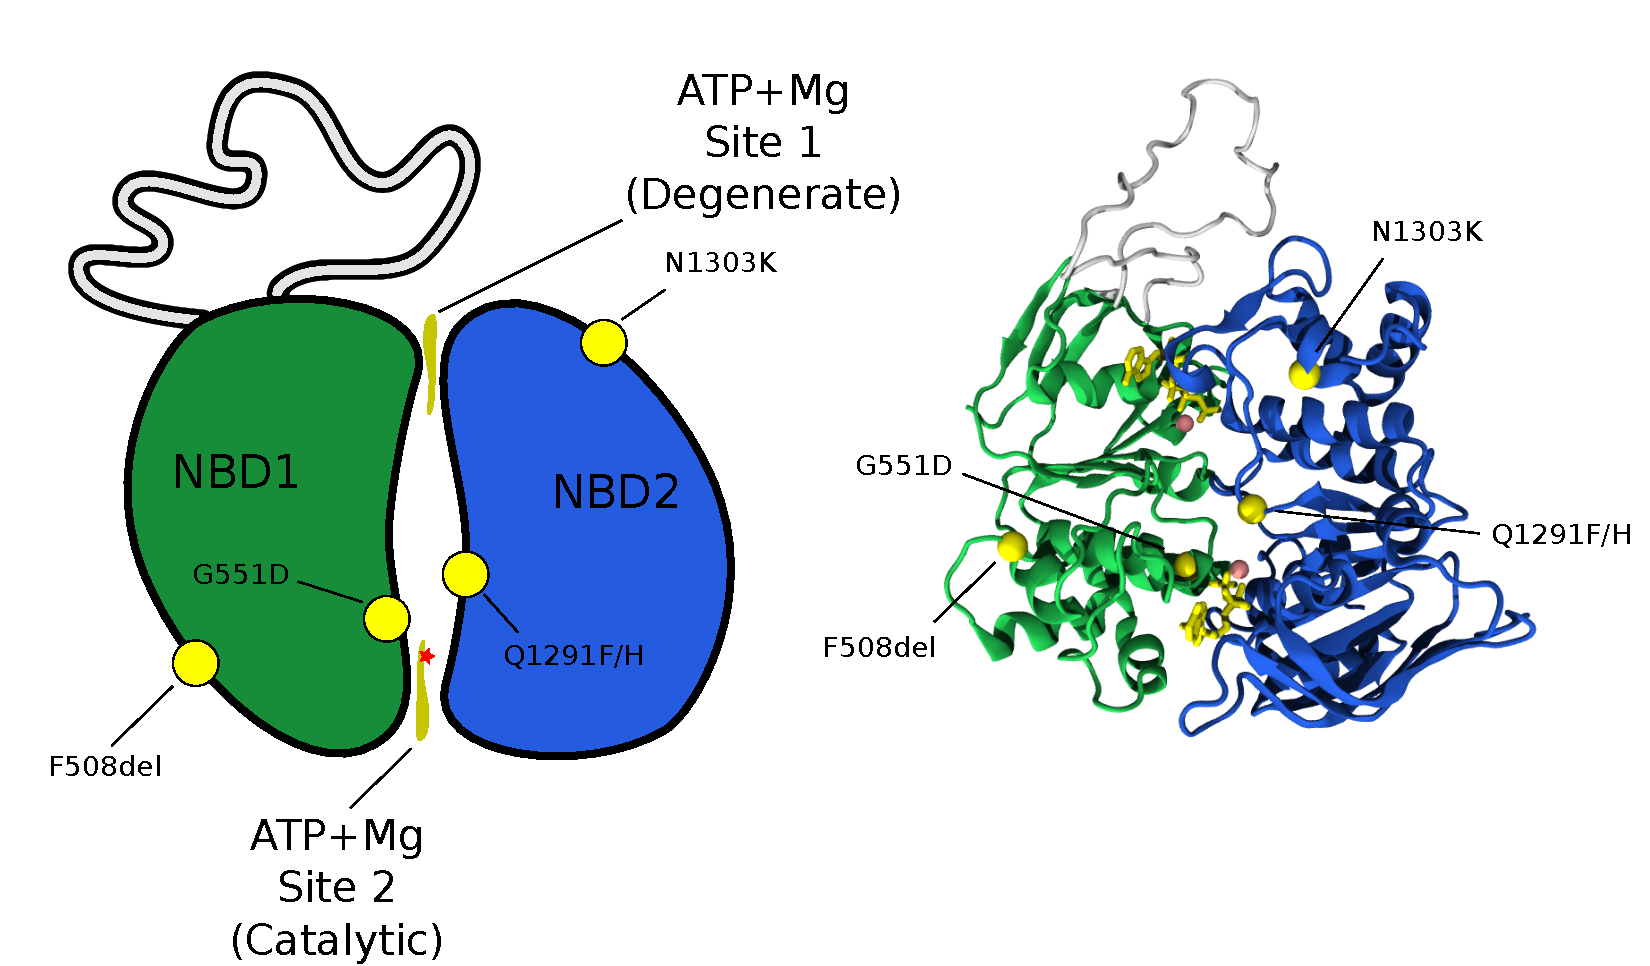
\includegraphics[width=0.8\textwidth]{figures/ATP_head_to_tail_figure.pdf}
	\end{center}
	\begingroup
	%\captionsetup{singlelinecheck = false, justification=raggedright}
	\captionof{figure}[NBD Organisation] {\textbf{NBD Organization}}{A) The NBDs are critical to the gating cycle of CFTR. They rest below the TMDs where they bind and hydrolyse ATP in order to regulate the gating cycle. B) Each NBD contacts both ATP molecules. This configuration is known as a head to tail dimer and is common amongst ABC transformers. One of the unique aspects of CFTR is the fact that only one of the ATP binding sites is capable of breaking down its ATP molecule through hydrolysis \cite{stratford2007}. When ATP is hydrolysed at site 2, the channel is allowed to close \cite{infield2021}. The regulatory insertion another unique feature of CFTR and has been shown to increase NBD1 stability when deleted. The  C) Molecular details of how the NBDs bind ATP at the two binding sites. Here we have highlighted several molecular details. The Walker A motifs are on both NBDs and are responsible for stabilising ATP in a conformation which allows hydrolysis to produce ADP and a phosphate group \cite{deltoro2016}. The Walker B motif on NBD2 is directly responsible for mediating hydrolysis, by allowing the movement of the magnesium cofactor \cite{urbatsch2000, rai2006}. Mutation of E1371 in Walker B is sometimes engineered to kill catalytic activity and lock the channel in an open state \cite{stratford2007, zhang2018}. Note the placement of both G551D, a gating mutation and Q1291H/F near site 2. The most common disease causing mutation $\Delta$F508 is located on a helix of NBD1 which buries itself into a hydrophobic pocket. N1303K is located at a roughly symmetric position on NBD2. } 

\label{NBD_structure}
\endgroup

The conformational transition from inactive to active differs significantly in CFTR compared to other ABC transporters. A transporter is characterised by acting as a gate to substrate, There is never a continuous path to allow the substrate to diffuse passed the protein. Since it is a channel, CFTR gives rise to a continuous pore \cite{linsdell2018}. 

CFTR's gating cycle is dominated by the action of the NBDs and the R-domain. The NBDs are largely similar are largely similar to other transporters in the ABCC subfamily so we will discuss them first. 

NBD1 and 2 each have two binding sites for an ATP$+$MG$^{2+}$ complex. This facilitates their dimerization in what is known a ``head to tail" configuration where both NBDs make contact with both bound ATP molecules \cite{gout2012}  (Figure \ref{NBD_structure}). Usually, in an ABC transporter the NBDs would contain contain a ``Walker A motif" to help them bind ATP \textit {and} a ''Walker B" motif to catalyse the hydrolysis. A unique aspect of CFTR is that NBD1 is missing its Walker B motif, meaning one of the ATP binding sites is incapable of hydrolysing ATP. This ATP binding site is sometimes referred as ``site 1", ''the degenerate site" or ''the non-consensus site" and it plays an important role in stabilising the open state of the channel \cite{yeh2022, csanady2019a}.

The other ATP binding site is referred to as ``site 2", ''the catalytic site" or the ''consensus site." The hydrolysis of ATP at this site triggers the closure of the channel. Sometimes, for the purposes of experiments, the catalytic activity of site 2 is intentionally halted through an engineered mutation. For example, E1371Q-CFTR is studied in structural determination experiments as it exhibits a much longer lived open state than the WT channel. This allows more snapshots to be taken of the open structure during cryo-EM experiments \cite{ramjeesingh1999, gout2012, muallem2009, hwang2013}. Indeed, the protein structure which was the source for our work carried this mutation and it had to be corrected to match the WT amino acid sequence before simulation \cite{zhang2018}. 

The above outlines the generally agreed upon chemistry about the action of the NBDs and gating. Beyond this there are some details about the gating cycle which are still up for debate. There are two competing models which give different predictions for how tightly coupled the dimerization of the NBDs is to the opening of the channel \cite{yeh2022}. The first proposed model is called the ``strict coupling model", which suggests that the NBDs and the TMDs rotate as rigid bodies, to move between the active and inactive states. This model would indicate that ATP binding and NBD dimerization is tightly coupled to the opening of the channel \cite{jih2012}. 

The second model is called the ``energetic coupling" model. This predicts that there are both closed and open states which are accessible while the NBDs are dimerized in the post hydrolytic state, as well as closed and open states while the NBDs are \textit{not} dimerized \cite{jih2012}. This means we would expect that we would expect the binding of ATP to be loosely coupled to the opening of the channel. It would seem that, although more complicated, the second model is both more consistent with recent findings in the literature and would also explain some of the other controversies surrounding the structure and function of CFTR, such as the strange, flexible conformation of TM8 \cite{fay2018}. These considerations are not critical for the work in this thesis but considering them in the future them may aid in targeted drug discovery efforts for CFTR, particularly for potentiator class drugs.

%allows nucleophilic attack by surrounding water on the phosphate tail of the ATP bound to site 2 B \cite{stratford2007}. Since the hydrolysis of ATP causes the channel to gate back to the closed conformation, mutations like E1371Q can be employed studied in contexts where one wishes to lock the channel in an open state such as structural determination 

Apart from the NBDs, the most important domain for the gating of CFTR is the R-domain. This disordered domain is unique to CFTR. In the inactive state the R-domain wedges between the TMDs, forming a plug and not allowing them to rotate to form a pore. Intermittently, Protein Kinase A (PKA) will bind to one of many segments on the R-domain coaxing the coils of peptide out into solution \cite{mihalyi2020}. PKA may then phosphorylate specific sites on the domain, causing it to remain in an unplugged configuration. It is currently unknown exactly how many phosphorylation sites there are in the R-domain, but more than 11 have been investigated \cite{mihalyi2020}. 

When the R-domain is phosphorylated it no longer rests between the TMDs. Rather, the amino acids which form the plug relocations to a site below the lasso motif. This was one of the main findings from chapter \ref{chap:I37R}. Further, in chapters \ref{chap:I37R} and \ref{chap:S945L} we demonstrate how the destabilisation of this binding site results in a gating defect.  

%\footnote{Note to physicists, phosphorylation is a process where a phosphate group is added to the side chain of an amino acid. Usually serine, tyrosine or threonine. This phosphate group a charge of -2, wheres these amino acids are normally neutral. This is a key regulator of protein activity as it places a very large charge at a normally neutral site in the protein.}


\subsection {Anion Selectivity}

\begin{figure}
	\begin{center}
	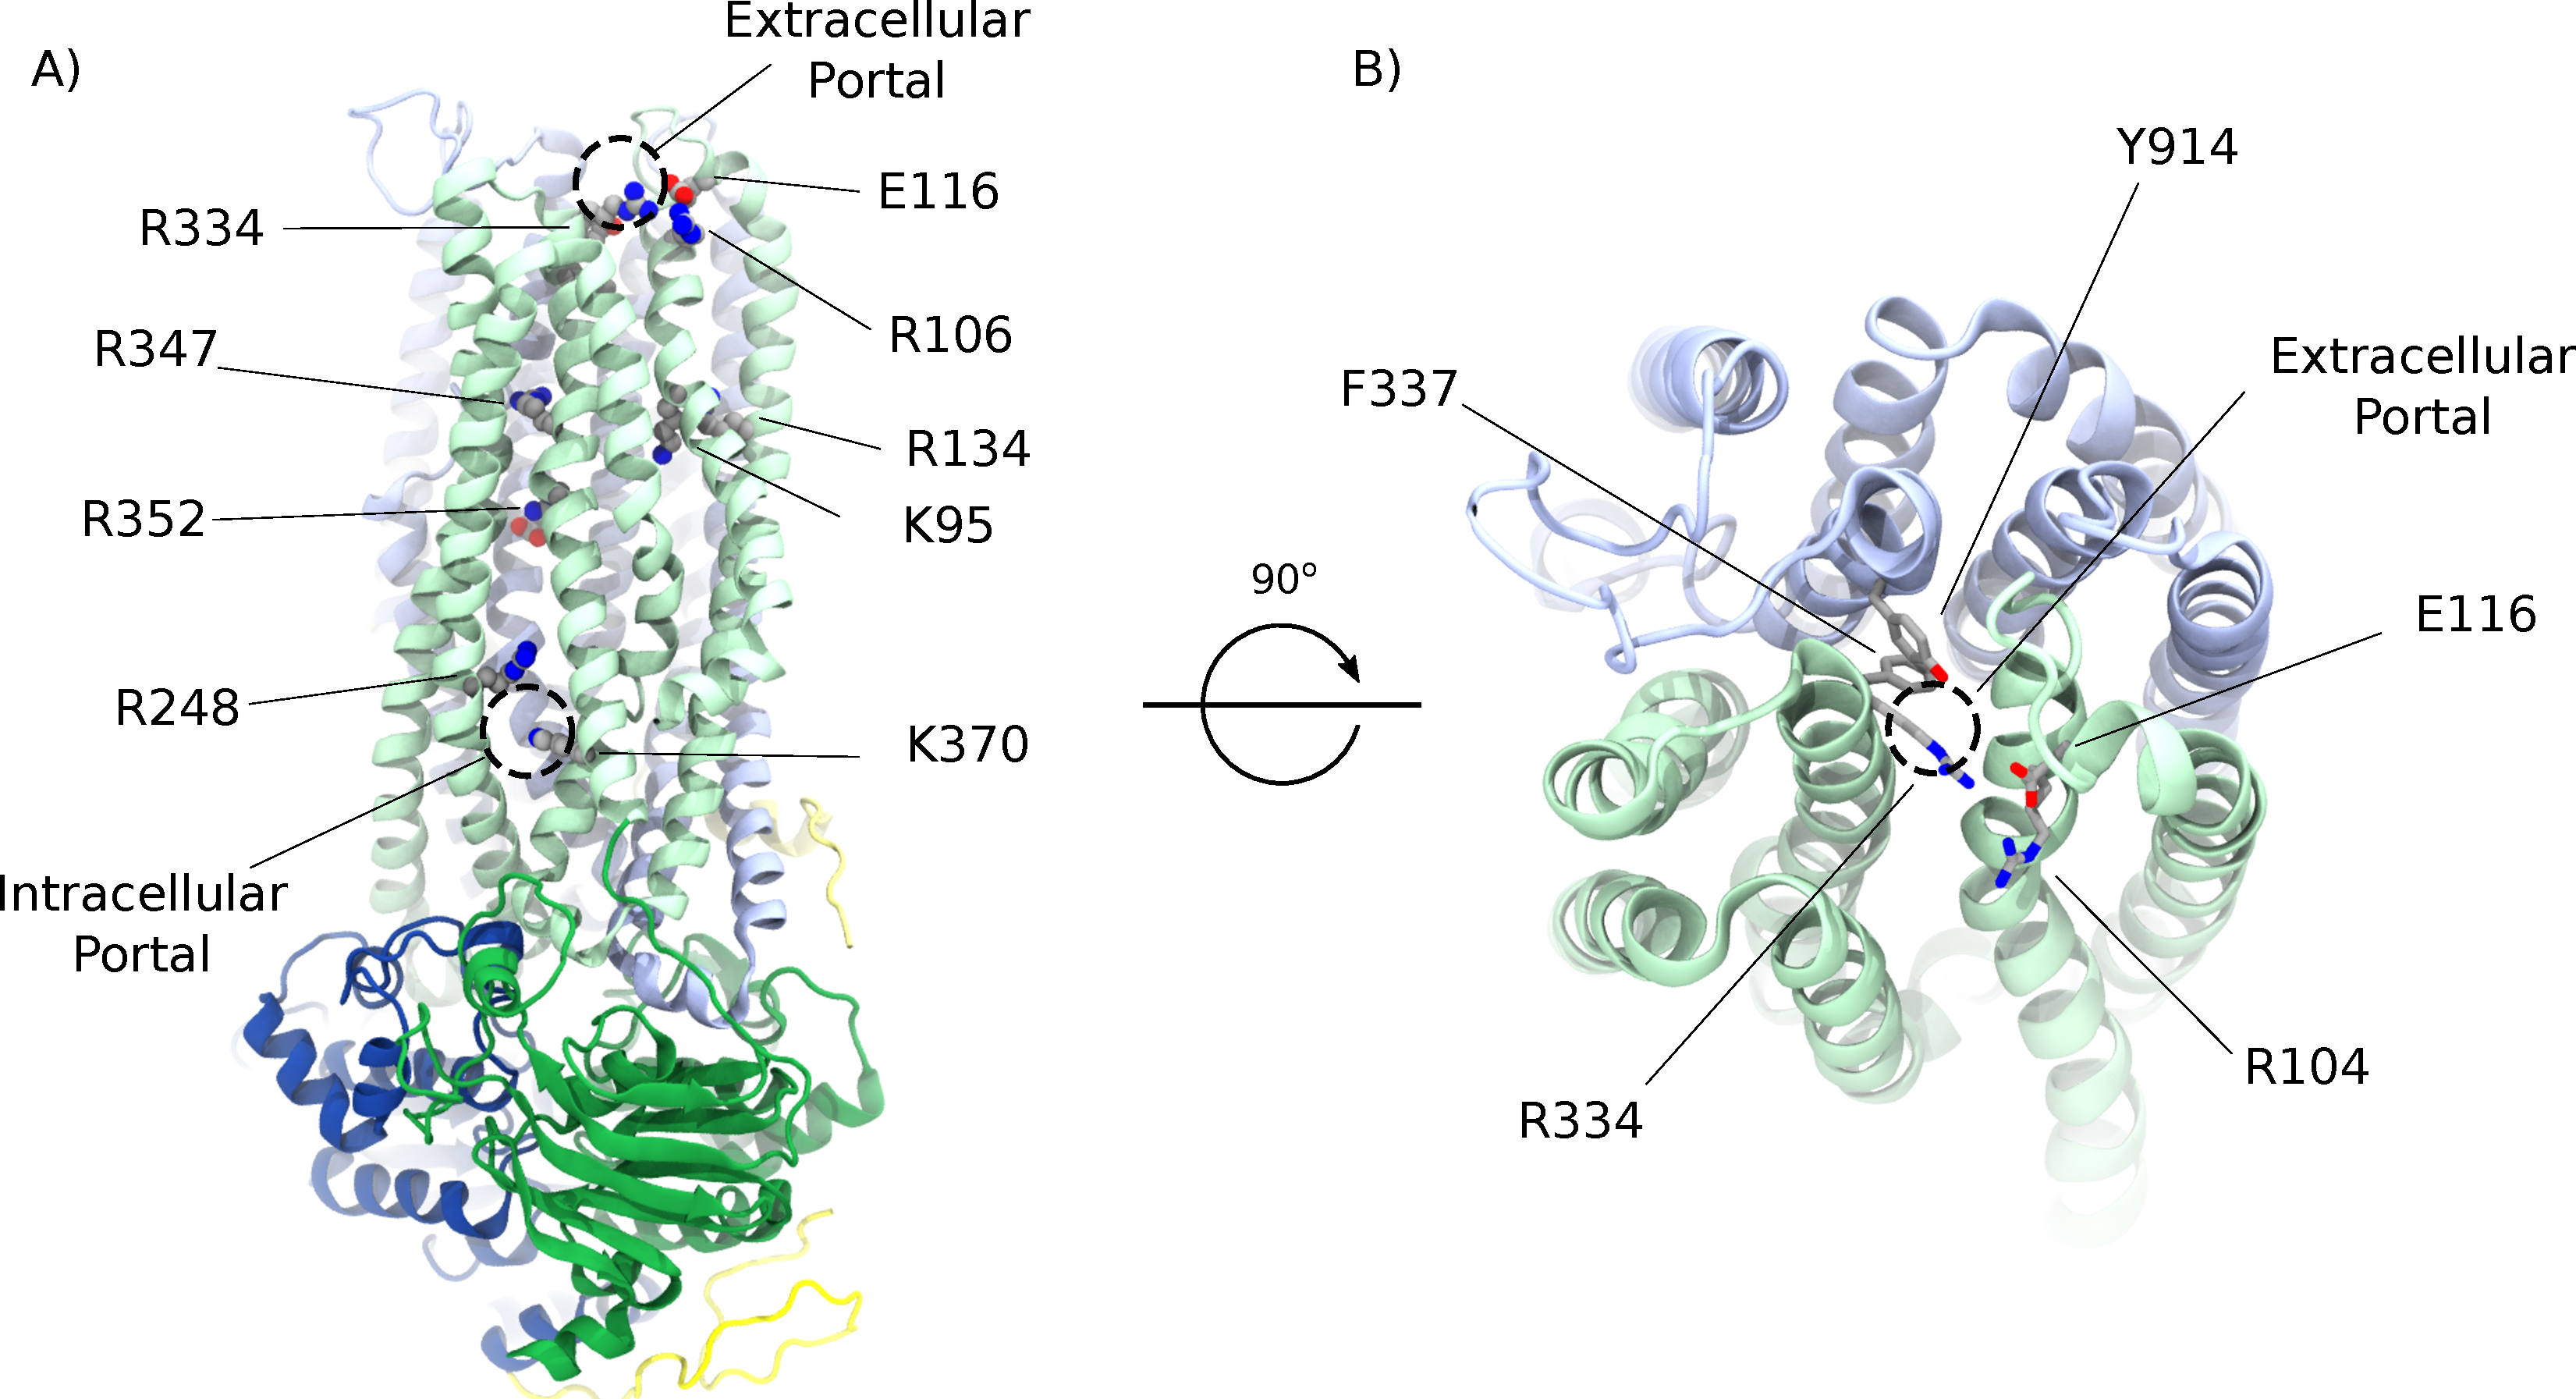
\includegraphics[width=\textwidth]{figures/chloride_passage_figure.pdf}
	\end{center}
	\captionsetup{singlelinecheck = false, justification=raggedright}
	\caption[Chloride Passage through CFTR] {\textbf{Chloride Passage Through CFTR}}{A)Ions enter through an intracellular gate, which is lined with positive amino acids. The subsequent inner vestibule is also lined with amino acids which chloride loosely associates with as it moves through the channel. B) A top down view of the extracellular portal. We have highlighted some hydrophobic amino acids which play important roles in the selectivity of anions. Pictured is the only available structure of the activated human CFTR channel \cite{zhang2018}. Unfortunately, this conformation is not sufficiently open to conduct ions. We will analyse an open conformation in chapter \ref{chap:opening} which we predicted through simulations.} 
	\label{chloride_passage}

\end{figure}

CFTR will not permeate cations but there are a set of anions which it will conduct. The conduction pathway of the channel can be split into two regions. The inner vestibule which is wide and covered with basic, positively charged amino acids and the selectivity filter which is formed by the narrowing of the protein in the upper part of the channel. These regions are hotspots for disease causing  mutations, with most mutations occurring on TM6 in TMD1 (Figures \ref{CFTR_mutations_pie_chart} and \ref{chloride_passage}) \cite{cftr2}. 

F337 is the most important amino acid for selectivity, with the F337A mutation leading to an increase in conductivity and a loss in selectivity \cite{wei2016}. Bicarbonate (HCO$_3^-$ is known to have roughly 25\% the permeability of chloride through the channel\cite{tang2009}. Some interaction partners such as WNK1 have been shown to influence the selectivity of the channel \cite{kim2019, garnett2011, kim2019a}. The permeation of bicarbonate is very important physiologically. If a CF-causing mutation permeates bicarbonate, there is a high likelihood the patient will be pancreatic sufficient. Increasing bicarbonate secretion is being explored as a possible therapeutic strategy \cite{ferrera2021}. 

Compared to cation channels like Gramicidin and KcsA, CFTR is only weakly selective---permeating a large set of anions with varying radii and geometries (Figure \ref{chloride_passage}) \cite{linsdell1998, tabcharani1997, poulsen1994}. CFTR appears to act like other anion channels where lyotropic (low solvation energy) anions pass more easily than kosmotropic anions (high solvation energy). This would suggest that partial dehydration of the anions is likely during conductance \cite{linsdell2000}. The radius of a dehydrated chloride ion is 1.7$\AA$ while a hydrated chloride ion has a radius of 3.2$\AA$ \cite{yang2002}. As noted in its source publication, the 6MSM structure which we have studied has a constriction of 1.2$\AA$ at its narrowest point. Hence, even if chloride were to be fully dehydrated during conduction, there would have to be some level of conformational change in the protein. This was the motivation for the extensive free energy calculations undertaken in chapter \ref{chap:opening}.

There have also been demonstrations that partially synthesised halves of the CFTR channel can dimerise to form chloride partially functional \cite{yue2000, ramjeesingh2003, cui2008, abbott2007}. The functional or therapeutic role this could play has not been explored.

\subsection{Different classes of Cystic Fibrosis Phenotype}
As the above shows, CFTR is a complex protein which can misfunction in a number of ways. Based on the way the mutation presents in \textit{in vitro} assays, disease causing mutations are classified into 6 common classes. Ultimately, the aim of this thesis is to demonstrate that that at the atomic level, there is much more nuance to these classes, and a mutation can have features of multiple classes at the same time.

This has important implications for the treatment of the disease. Due to the heterogeneity between patient responses to therapies, there is a growing interest in personalising the treatment of disease and mapping the molecular effects of mutations can inform this process of theratyping \cite{crawford2018,sette2021}. As patient specific treatment evolves, these classes will likely become less relevant, serving as illustrative tools only to communicate at a higher level what is going wrong with the CFTR protein. The specific choice of treatment will depend on a number of personal factors. The canonical classification is as follows:

\begin{figure}
	\begin{center}
	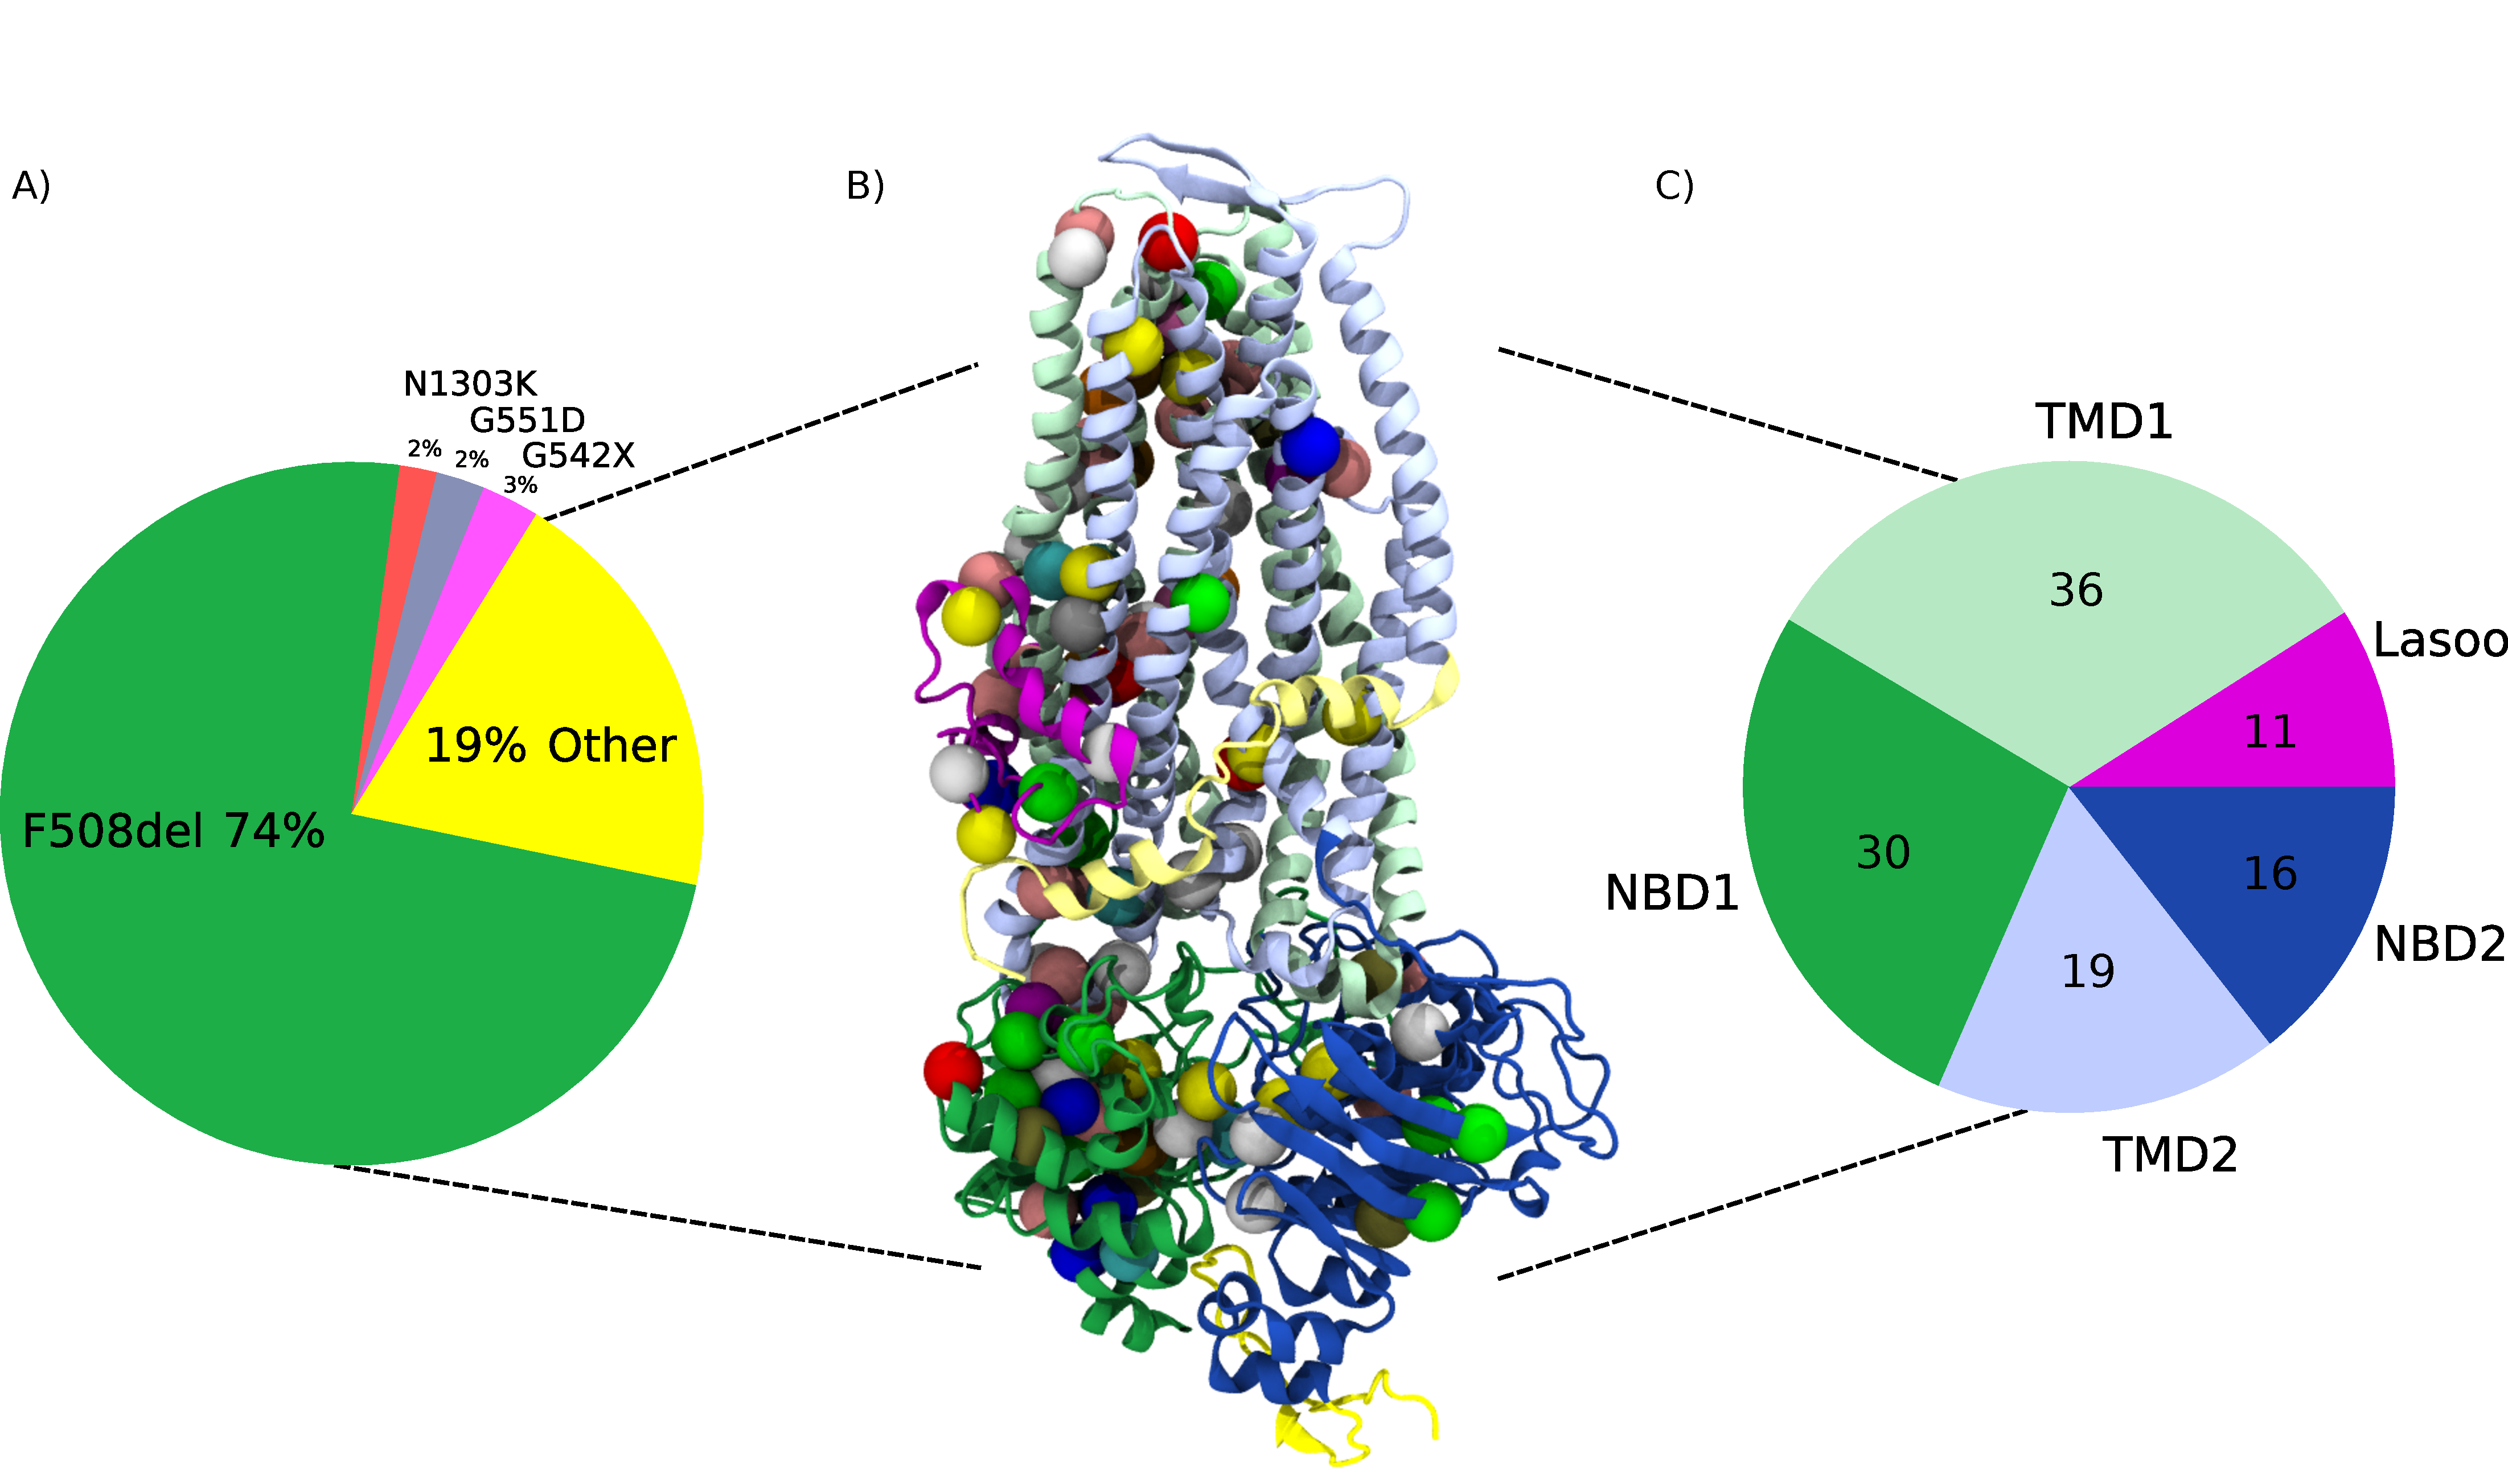
\includegraphics[width=\textwidth]{figures/alleles_pie_chart.pdf}
	\end{center}
	\captionsetup{singlelinecheck = false, justification=raggedright}
	\caption[Rare Mutations Occur in Across the CFTR Protein] {\textbf{Rare Mutations Occur in All parts of the CFTR Protein}}{A) The reported frequency of all disease causing alleles (not just missense mutations) in the CFTR2 database. At the time of writing there are 402 recorded different disease causing mujtations. A patient with CF will carry two of these mutations. 1 in 25 people of Northern European descent are a carrier for CF and are themselves at increased risk for many health problems \cite{ioannou2014, miller2020}. B) The location of all 112 known disease causing missense mutations mapped on the CFTR protein itself as spheres. In addition to those visualised here there are many of variants of unknown significance (VUS) which may cause disease but are so rare they have not been clinically studied. C) The incidence of CF causing missense mutations in the different domains of the CFTR protein. TMD1 and NBD1 have the highest concentration of disease causing mutations. Likely due to the former's role in ion permeation and the latter's role in gating \cite{cftr2}}. There are no confirmed CF causing missense mutations in the C-terminus or the R-domain. As patient registries are set up across the world it is likely that more rare CF causing mutations will be discovered in the future. \footnote{Note that in this figure we have included the novel I37R mutation studied in this thesis. This mutation has not yet been recorded in CFTR2.} 
	\label{CFTR_mutations_pie_chart}
\end{figure}


\begin{itemize}

	\item \textbf{Class I} No functional protein. Under these mutations no protein is transcribed due to either problems with the transcription of mRNA or a premature stop codon truncating protein synthesis early, meaning the resulting peptide is missing key domains. 
	\item \textbf{Class II} Folding defect. These mutations cause the translated peptide to misfold into the incorrect tertiary structure. This can inhibit the protein's journey as it is trafficked to the cell membrane. 
	\item \textbf{Class III} Impaired Gating. Here the mutation inhibits the ability of the protein to transition from the closed to the open state. 
	\item \textbf{Class IV} Decreased Conductance. These mutations cause a barrier in the energy landscape of the CFTR chloride conductance pathway.
	\item \textbf{Class V} Less Expressed Protein.  
	\item \textbf{Class VI} Decreased Functional Lifetime

\end{itemize}

Although useful from a clinical and experimental standpoint, in reality, these classes do not reflect the molecular nature of a mutaiton. Mutations may in fact belong to many categories at once, to differing degrees. This has lead to a more granular approach in more recent literature \cite{veit2016}. In particular, through this thesis we will demonstrate that membership of one of these classes can be due to a range of molecular phenotypes. Hence, this classification is becoming increasingly outdated and there is a need to understand the unique, sometimes overlapping, molecular phenotypes of each mutation. Further, through our molecular simulations we will see that in fact CFTR modulators appear capable of treating many different mutations with unique modes of pathogenesis. This is the purpose of chapters \ref{chap:I37R}-\ref{chap:opening}. In each chapter we will analyse a specific mutation in detail and then use \textit {in vitro} techniques to demonstrate that the molecular defect introduced by the mutation can be rescued by existing CFTR modulators. 

A molecular understanding has previously been outlined for certain mutations, though rarely with the advantage of the full hCFTR structure or extensive statistical sampling. For example, \cite{belmonte2015} based their modelling on SAV1866 and used short unbiased simulations as well as simple free energy estimates in order to demonstrate the deleterious nature of the G551D and $\Delta$F508 mutations. This is remarkably consistent with the findings of more recent studies which have the benefit of more structural information about the protein \cite{bahia2021}. This latter study used isolated structures of NBD1 and 2 (PDB IDs: 2PZE \cite{atwell2010} and 6UK1 \cite {wang_2020_nbd2_CFTR_isoalted_pdb_alone} respectively) in order to predict the $\Delta\Delta G$ change to the folding energy of CFTR from disease causing mutations. The authors correlated their results with \textit{in silico} prediction functions from Rosetta and find remarkable agreement. Although this study does not shed light on molecular details of misfunction, it will likely be a critical resource for the grouping of theratype. 

To date, there are two studies which have used a similar approach to us to study mutations. They also attempted to understand the molecular defects of rare mutations \textit{in silico} and then combining these findings with patient specific platforms to demonstrate their rescue by CFTR modulators. The first of these studies used the zCFTR structure, in order to study the ultra-rare W361R mutation \cite{billet2020}. Here, the authors found that a lipid tail binds into a hydrophobic pocket formed by the W361 amino acid. This lead to the expectation that the W361R mutation would cause a class II folding defect. Unfortunately, the authors did not explicitly simulate the effects of the W361R mutation, though the nature of the folding defect they would expect to see is likely not accessible on simulation time scales.

A second study addressed the intriguing mutation P67L on the lasso motif \cite{sabusap2021}. This mutation occurs in a hotspot of CF-causing mutations and also in the vicinity of corrector type drugs \cite{gene2008, fiedorczuk2022}. Here, the authors were able to rely on the structure of activated hCFTR to  a change in NBD2. However, the simulation methodology in this paper is questionable. The authors simulated hCFTR for less than 200ns and claim to have discovered allostery between the lasso motif and NBD2. Such an effect would likely take orders of magnitude more simulation time to observe because of the distance between these domains in the simulated structure. The simple statistical test employed by this paper in Figure 7, on a single simulation replicate, is also not fit for purpose \cite{knapp2018}. However, the pharmacological and biochemical results from this publication are certainly extremely successful in shedding light on the molecular nature of this mutation.

Although the authors of these works have seen the deleterious effects of mutations through simulations and demonstrated their rescue with pharmaceuticals, these prior studies are not as rigorous as the work we have undertaken for this thesis. None of these studies simulated CFTR for more than 1 microsecond and none of them have employed free energy calculations. However, these study validate the approach we will use for subsequent chapters and further, allow us to demonstrate the power of using MD and free energy calculations as computational microscopes to investigate CFTR misfunction. 

Similar to the above, the defects we will explore in each chapter are largely unique: 

\begin{itemize}
	\item \textbf{I37R} is a mutation which occurs on the lasso motif. In chapter \ref{chap:I37R} we explored how this novel mutation causes a class III gating defect by giving rise to a pathogenic interaction with a fragment of the R-domain. This fragment was poorly resolved in the cryo-EM structure of CFTR and we first had to identify it using MD. Our structural predictions were then confirmed upon the release of Alphafold2 \cite{jumper2021}.  

	\item \textbf{R352Q} deletes a positive charge on TM6, along the chloride conduction pathway in the inner vestibule. In chapter \ref{chap:R352Q} we used umbrella sampling and unbiased MD to demonstrate the misregulation of the conduction pathway in this mutation. Demonstrating a class IV conductance defect. 

	\item \textbf{S945L} occurs in TM8 on TMD2. In chapter \ref{chap:S945L} we discovered a stable network of hydrogen bonds which links S945 to Y852 on the R-domain. We hypothesised that the replacement of the polar serine sidechain with hydrophobic leucine might cause a perturbation to this section of the R-domain. Due to the kinetic barrier from the surrounding lipids we again employed umbrella sampling to explore how the perturbations this mutation causes to the R-domain causes both a folding and a gating defect.

	\item \textbf {R334W} occurs at the extracellular pore, at the end of the selectivity filter on TM6 in TMD1. In chapter \ref{chap:opening} we used multiple walker OPES-metadynamics in order to dilate the existing structure of human CFTR (PDB ID: 6MSM) and study the effects of the R334W mutation on chloride conductance.

\end{itemize} 


Through our MD simulations, we found that each of these rare mutations has a unique molecular fingerprint. They appear to cause CFTR to misfunction in unrelated ways. Further, in each of these cases, we have either presented \textit{in vitro} patient specific assays or surveyed the literature to demonstrate that pharmacological rescue of these rare mutations is possible using CFTR modulators \cite{R334W_Euro_CF_trial}.  It is then remarkable that these unique molecular modes of pathogenesis all to respond to CFTR modulators. It is these results which inform the conclusions in chapter \ref{chap:conclusion}, where identify directions for further studies of CFTR and argue that many patients who are currently excluded from access to modulator therapy are likely to benefit from these life changing drugs. 

%FIGURE demonstrates how each of the canonical classes at the molecular level is broken down into many sub classes and a mutation might belong to one of many of these subclasses. Structural biology paradigms and \textit{in silico} modelling can help classify mutations into these different classes. In combination with wet lab assays we can understand which classes of these molecular defects are most effectively treated with specific drug regimens. Our computational microscope is helping choose treatments for patients at the atomic level. 

\section{Modulators Act Directly on CFTR to Restore its Function}
\begin{figure}
	\label{drugs_bound}
	\begin{center}
		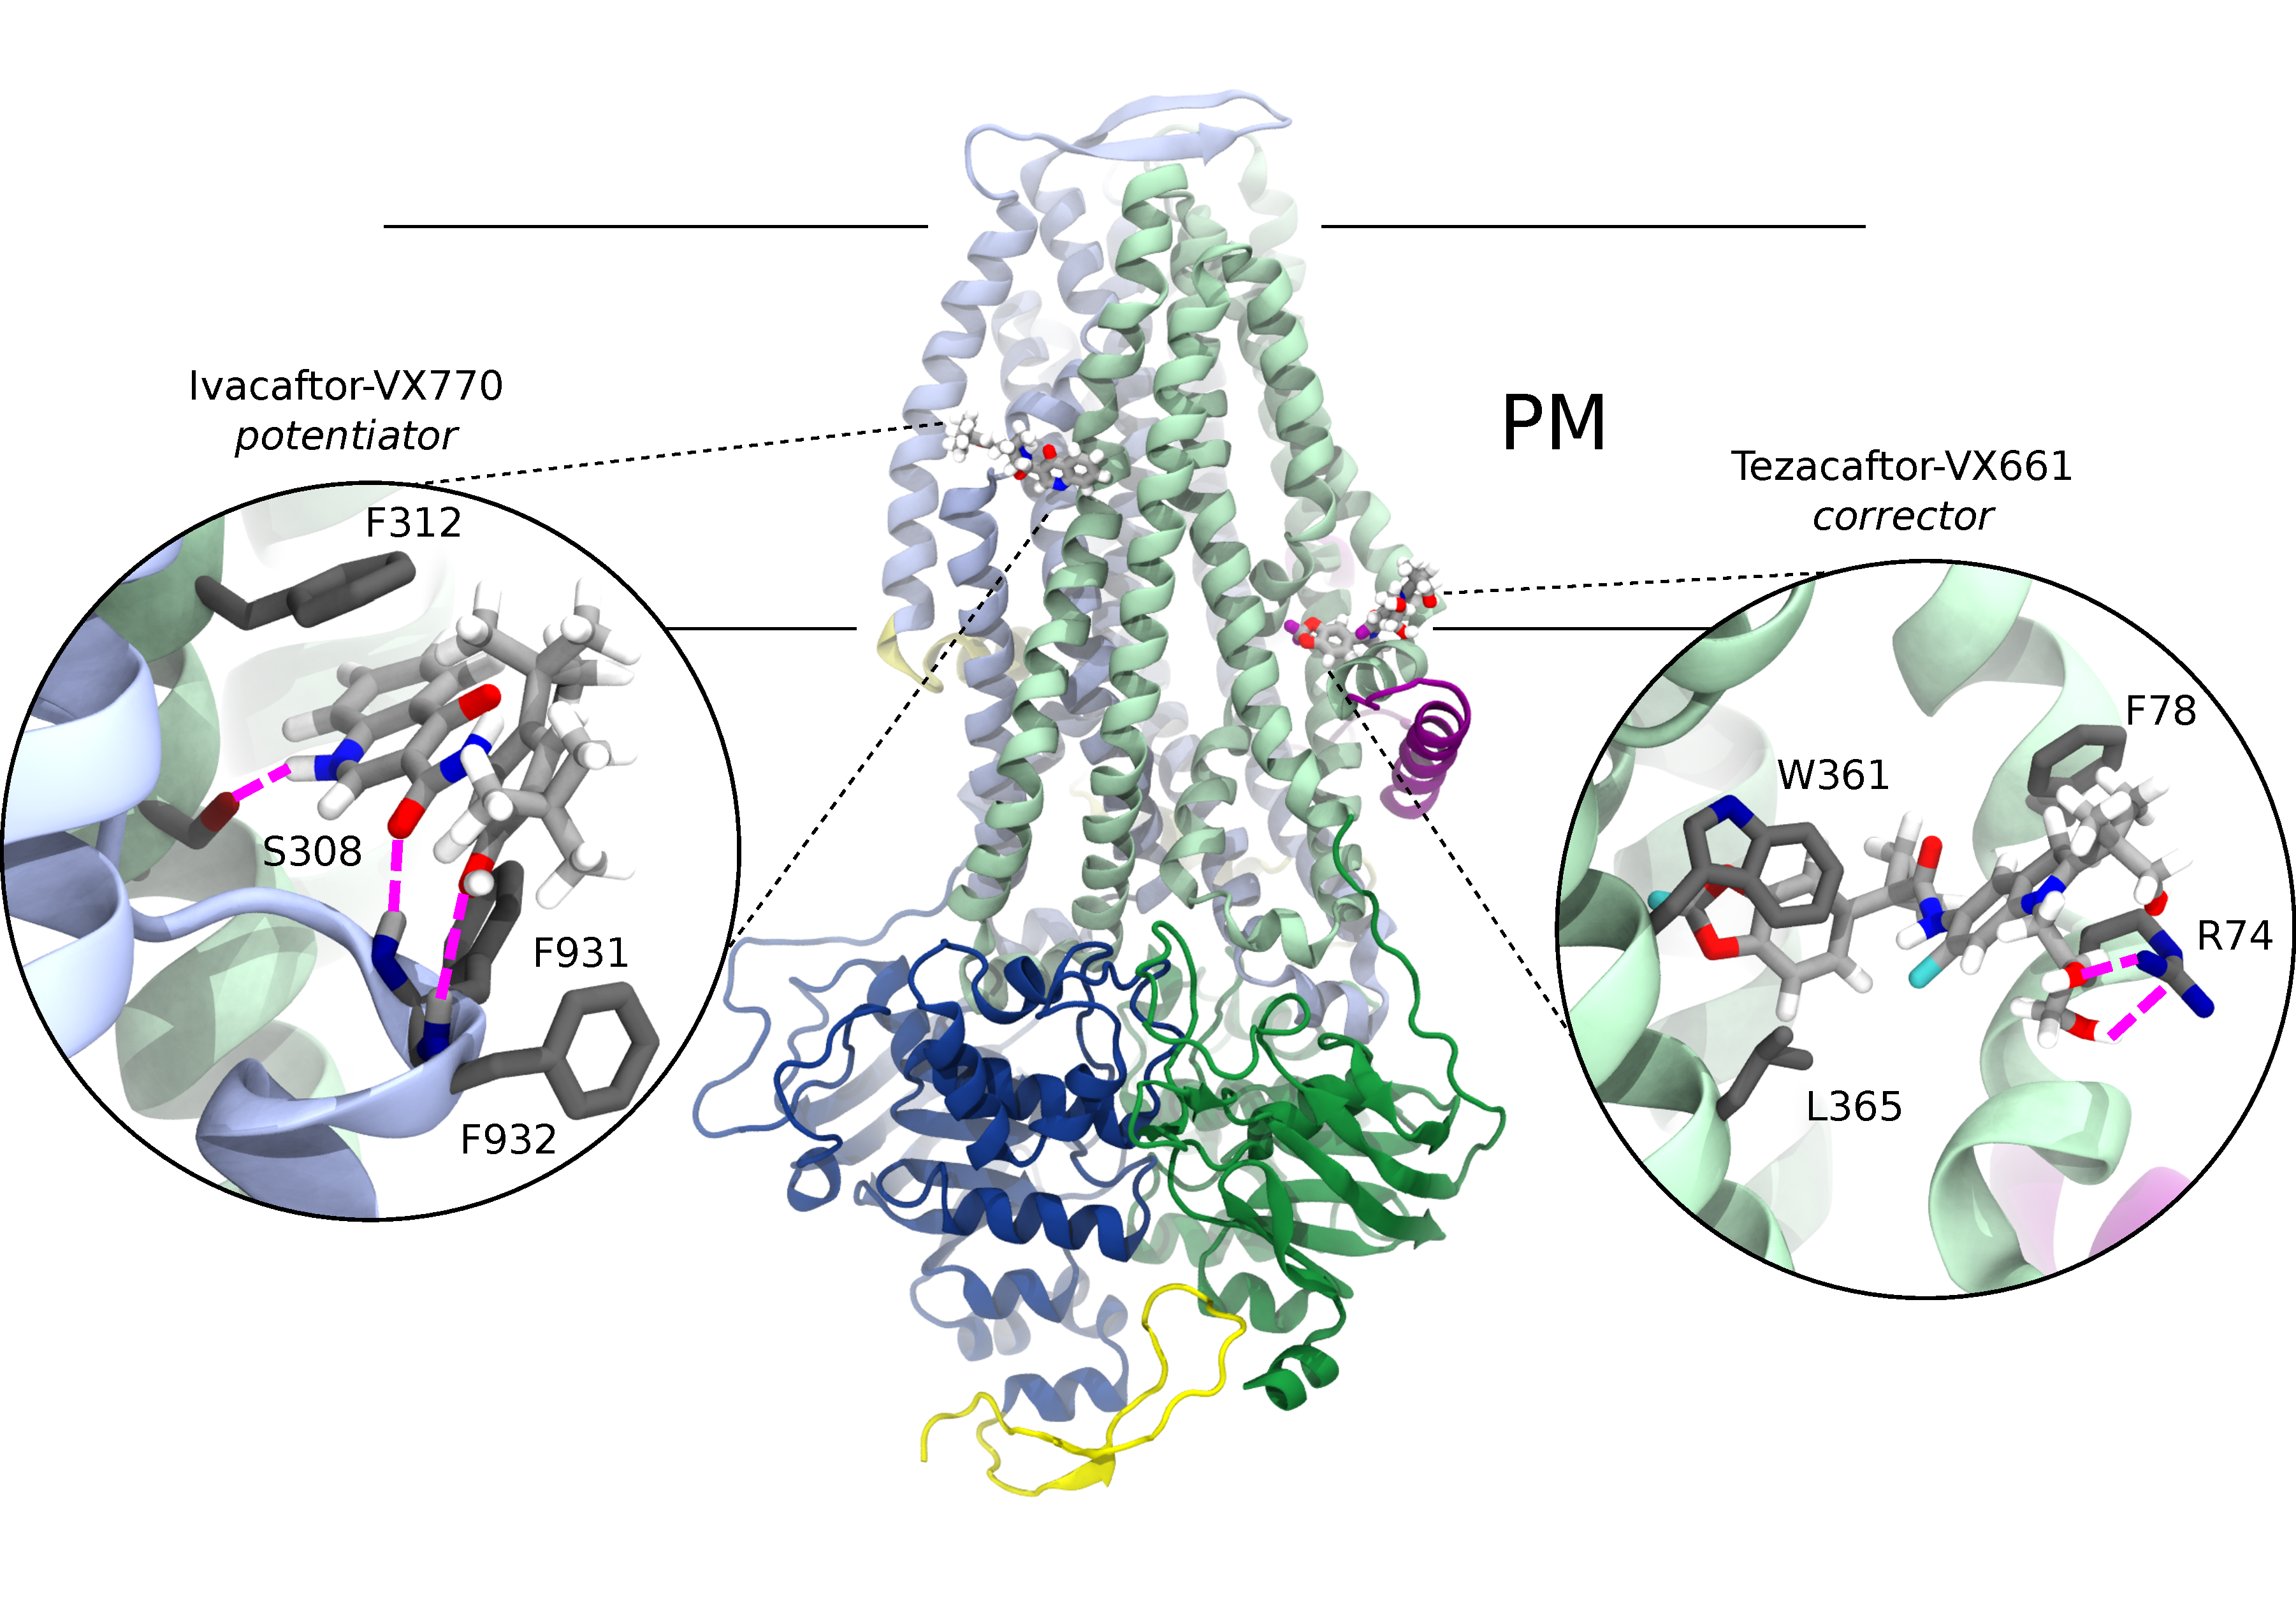
\includegraphics[width=1\textwidth]{figures/drugs_bound_overall.pdf}
	\end{center}
	\captionsetup{singlelinecheck = false, justification=raggedright}
	\caption[Modulators Bound to CFTR] {\textbf{Modulators Bound to CFTR}}{The structurally imaged binding sites of potentiators and type I correctors \cite{liu2019, fiedorczuk2022}. Potentiators in particular are proposed to bind to other sites as well \cite{yeh2019, liu2019}. Hydrogen bonds are labelled with purple dotted lines. Note how both visualised binding sites require substantial contributions from the surrounding lipid bilayer. The presence of these lipids will play an important role in the binding kinetics and energetics of these drugs \cite{csanady2019}. Future molecular studies should account for these nuances.} 
\end{figure}

Since CFTR is at the heart of CF pathogenesis, it has been pursued for decades as target for therapeutics. Through high throughput \textit{in vitro} screening, four compounds which act directly on CFTR have been clinically approved for the treatment of CF. These drugs are known as CFTR modulators. They fall into two categories. Correctors, which aid CFTR to fold into the correct state and potentiators which help the channel reach the fully open state once it has folded correctly and integrated into the membrane. Since their discovery, several \textit {in vitro} biophysical experiments have investigated the mechanism of action and binding site of these compounds \cite{csanady2019,  laselva2022, yeh2017, yeh2019, fiedorczuk2022, krainer2018}. 

Due to the excitement surrounding these compounds, there have been a few simple \textit{in silico} studies of CFTR modulators\cite{molinski2018, bitam2021, baatallah2021, froux2020}. When not performed carefully, \textit{in silico} docking studies for small molecules may produce very crude and inaccurate findings, this was particularly apparent when reviewing the large number of docking studies performed during the coronavirus pandemic of 2020-2022 \cite{gimeno2019, derek_lowe_virtual_screening_2022, ceron-carrasco2022}. It is then fortunate that previous MD and docking studies of CFTR modulators have been largely consistent with subsequent structural and biochemical experiments \cite{liu2019, scientifique2019, yeh2019, yeh2017, fiedorczuk2022}. Even though these studies are limited in the impact of their findings, their success can be attributed to the close integration of these \textit{in silico} techniques with biochemical assays. This would indicate some promise for the approach of this thesis and future \textit{in silico} studies of CFTR which, will hopefully have access to even more computational power and structural information. 

%Recently, cryo-EM structures of many of these compounds in their bound state have been published \cite{liu2019, fiedorczuk2022}. 

An added benefit of modulator therapy is that they have have demonstrated promise in improving not just the most acute symptoms of CF (lung function), but they may be able to treat or even relieve deleterious CF associated complications. In some cases, modulators have been found to relieve pancreatic insufficiency and CF related diabetes \cite{gaines2021,lopes-pacheco2020, yi2021} and there is ongoing ongoing study into the possible benefits of modulators on bacterial infections \cite{harvey2022}. This highlights the importance of treating the root cause of a disease when we are presented the opportunity and not just its symptoms. 

\subsection{Correctors}
Corrector class modulators are able to treat Class II folding defects. The most common type of correctors are known as type I correctors, which help the CFTR protein fold into the correct structure by binding to a hydrophobic pocket in TMD1 formed by TMs 1, 3, 4 and 6. This binding mode has been directly visualised by cryo-EM imaging with atomic resolution \cite{fiedorczuk2022}. This binding mode was expected, as circular dichromism \cite{greenfield2006} and fluorescence experiments found that an isolated construct of TMH3 and TMH4 were more likely to fold correctly in a model membrane in the presence of corrector compounds \cite{krainer2018}. 

In combination, these studies give us a strong base to understand the mechanism of action for corrector compounds. The correctors tezacaftor (VX-661) and elexacaftor (VX-445) form two components of the triple therapy Trikafta \cite{administration2021, trikafta_website}. Tezacaftor is a type I corrector while elexacaftor has been found to have some potentiation capacity on CFTR, leading it to be classified as a type III corrector. A review of all types of correctors can be found in \cite{veit2018}. Further work will aid in the creation of new compounds to refine our exploitation of current correction strategies.

\subsection{Potentiators}
Potentiator class drugs bind to CFTR in order to increase the number of channels which are conducting chloride in the cell at any one time. This helps to balance osmotic pressure over the epithelium and relieve symptoms \cite{fda_kalydeco_2_years_or_older, fda_kalydeco_approval, jih2013,yeh2017}. However is some uncertainty surrounding the molecular details of their mechanism of action. 

There is consensus that potentiators bind directly directly to CFTR, in order to increase the likelihood that the channel occupies a conducting state. Indeed, some potentiators such as VX-770 (ivacaftor), which forms the third component of Trikafta, rescues CFTR with picomolar affinity \cite{csanady2019}. 

Controversy arises surrounding precisely \textit{where} these drugs are binding in order to rescue CFTR. Different studies discovering different binding sites for the same drugs, via mutagenesis and other methods \cite{yeh2019, liu2019, laselva2021}.  

Careful investigation of different potentiator molecules give hints as to the solution to these problems. For example, GLPG1837 has not been approved in a clinical setting but through \textit {in vitro} experiments it has been demonstrated that it is more efficacious at potentiating CFTR even though it has lower affinity for the CFTR protein itself \cite{vanderplas2018}. This would indicate that the highest affinity binding pocket does not produce the greatest modulation. 

More work is needed to resolve the mechanism which results in the highest clinical effectiveness of these drugs. These disagreements are closely related to the kinked conformation of TM8, where they are proposed to bind \cite{liu2019, yeh2019}. Some of these issues will be addressed in more detail in chapter \ref{chap:conclusion} where we will suggest some \textit{in silico} strategies to address them. 

The competitive nature of certain potentiator and corrector drugs opens the possibility that specific genetic defects may be optimally rescued by specific combinations and doses of both correctors and potentiators compounds \cite{csanady2019}. This means there may be much to gain from the patient specific approach like the one employed for this thesis. 

The elucidation of the binding site for potentiators has been attempted with unbiased MD using the hCFTR structure (6MSM) \cite{laselva2021}. This study used an octanol slab as well as a model POPC membrane in order to accelerate the diffusion of VX-770 in the transmembrane portions of CFTR. With 10 $\mu$s of unbiased MD sampling, the authors discover 7 binding poses for the potentiator drug. The authors combine their results with a photo-label and mass spectrometry results which will likely play a critical role in future drug development of potentiators. They use these innovative toosl to conclude that both a site on ICL4 and the site visualised by cryo-EM experiments play a role in potentiating CFTR activity. This is consistent with other \textit{in vitro} experiments \cite{csanady2019}.

Unfortunately, in this study, none of the binding sites observed \textit{in silico} corresponded to the binding mode visualised by cryo-EM experiments \cite{liu2019}. The authors speculate that this may be because the cryo-EM site is in fact low affinity but it is likely that even though 10 $\mu$s is represents a considerable investment of computational resources, it is simply not enough sampling to see ligand binding and unbinding. The kinetics of a membrane facing drug binding site occur on the order of milliseconds \cite{weikl2016}. Hence, free energy calculations would be needed for such an endeavour and we will propose such a study in chapter \ref{chap:conclusion}. 

\subsubsection{Read Through Compounds}
Roughly 10\% of known disease causing mutations result in a premature stop codon in the mRNA of the CFTR gene. This means protein synthesis is stopped early, and the resulting protein will be missing critical domains. 

Since there is no full length CFTR protein synthesised by cells carrying this mutation, potentiators and correctors are unable to directly assist. This has lead to the need to develop a class of drugs known as read through compounds which allow the continued synthesis of the protein, past the premature stop codon \cite{sharma2021}. At the time of writing no read through compounds have been clinically approved but efficacy has been demonstrated in pre-clinical models \cite{crawford2021}. Since correctors and potentiators also modulate the behaviour of WT-CFTR it is likely that correctors and potentiators would be given in combination with read through compounds and other therapies as a complimentary treatment.

\subsubsection{Alternative and Complimentary therapeutic Strategies}
As the root cause of disease, CFTR will continue to be an important therapeutic target. However, there will also be increasing value in the therapeutic benefit derived from manipulating other protein systems---both as complimentary a strategy to the modulation of CFTR and to the treatment of complications. This is especially pertinent when we consider that some patients do not respond to CFTR modulators, even when they share the genotype of patients who do. These patients would benefit greatly from complimentary therapeutics \cite{hanafin2021, robertson2015, lingam2017, seelig2020, barbieri2021a, grebert2019}. 

As mentioned in section \ref{clinical_realities_CF}, one of the most troublesome complications of CF is the chronic infection experienced by patients. Unfortunately, modulators have not been able to reliably alleviate this complication \cite{mallapaty2022}. This is because these bacterial colonies a protective biofilm and thus become very difficult to eradicate with traditional antibiotics. To this end, bacteriophage therapies are being pursued as a complimentary strategy to those above \cite{ng2021}. 

There is also exciting work on gene and cell based therapies to directly deliver properly functioning CFTR proteins into the bodies of CF patients \cite{allan2021}. This is being investigated through the use of different advanced vectors, such as the retro virus lentivirus. With these vectors, WT-CFTR is usually added \textit{ex vivo} and then the treated cells are transplanted back into the patient. However, it may may soon be possible to edit the genome of a CF-afflicted embryo and cure the patient before they are even born using a system like Crispr-Cas9 \cite{ledford2020}. This latter technique has been misused in the past \cite{mallapaty2022} and the reader is again referred to section \ref{cftr_lit_review_intro} for texts on bioethics. 

\section{Patients with Rare Mutations Struggle to Access Modulator Therapy}
CFTR modulators have proven to be a breakthrough in the treatment of CF. However, there is strong motivation behind our focus on rare mutations in this thesis. Roughly 50\% of Cystic Fibrosis cases are caused by a homozygous mutation, $\Delta$F508, and 90\% of patients carry at least one copy of this mutation. At the time of writing, many jurisdictions such as Australia and the EU have approved a drug combination therapy known as Trikafta for patients carrying one copy of $\Delta$F508. Given that these drugs act directly on CFTR, we would expect that mutations may also respond to triple therapy. 

Thus, the exclusion by regulators of patients with rare mutations leaves a significant part of the CF afflicted population without access to this life saving medication, with many more excluded due to the extreme cost of the drugs themselves \cite{administration2021, trikafta_website, abdallah2021, guo2022a}. 

Traditional clinical trials are also not possible for many of these rare mutations, as there may not be enough patients carrying one mutation to study them in the same trial \cite{grody2007}. Hence, we aim to demonstrate that a larger section of the CF population is likely to respond to modulators, particularly those carrying missense mutations. Eventually this work will contribute to a clinical method known as theratyping, where a granular understanding of CF pathogenesis will allow a personalised choice of treatment.

The treatment of rare mutations has particular significance in CF. Not only would patients be otherwise left behind, but by studying rare mutations, outcomes can be improved for all people with CF. For example, potentiator class drugs were discovered by high throughput molecular screening against the rare class III gating mutation G551D \cite{vangoor2009}. By studying rare mutations we can gain a more complete understanding of the nature of the disease and so improve therapies for everybody. This approach will become more important in the future as CF is uncovered in regions where it is rarer. In these populations there is also a broader spectrum of CFTR mutations, meaning patients in these regions are more likely to have a rare form of disease \cite{singh2015,zheng2017,ni2022}. As patient registries are launched in these populations, we will discover more rare forms of CF. This expected trajectory of CF epidemiology makes the approach of this thesis critical, such that all people with CF can benefit from the advances being made by translational research \cite{zheng2017, garcia2022}. 


%Patients with rare forms of CF are more likely to be in countries where CF is already quite rare \cite{zheng2017}. Patients on modulators have significantly different clinical outcomes even between those with the same genotype. Determining the reason for this would open the door to the development of complimentary therapeutics. 

The earlier patients are able to benefit from modulator therapy, the better their prognosis \cite{lahiri2022}. It is also well documented that patients with the same genotype may respond differently to the same modulators \cite{hanafin2021}. Hence, by validating a patient specific approach to rare mutations we can build a platform to choose the right modulators for all patient. Considering that patients with the same genotypes often respond differently to the same modulators, it is critical that more modulators and complimentary therapies are developed, to give all patients more options and better outcomes \cite{hanafin2021}.

\section{Patient Derived Organoids: A Pre-Clinical Model to Assess Modulators}
In chapter \ref{chap:methods} we constructed a model based on interacting atoms to study biomolecular systems. Similar to this philosophy, medical researchers also seek model systems to understand the function of organs. In CF research, this has lead to the development of techniques where samples of epithelial stem cells are taken from patients and grown into structures which mimic the function of either the lung or the gut \cite{wong2015,depoel2020}. These are known as patient derived organoids.

This is possible due to a population of adult stem cells which live in the epithelium. These cells maintain their ability to differentiate into a variety of cell types (a property known as pluripotency) \cite{blanpain2007}. 

To grow organoids, epithelial stem cells are scraped from a patient's nasal passages or taken during a rectal biopsy. These samples can be used to grow either lung or intestinal organoids respectively  \cite{awatade2021,sato2011}. The morphology of the organoids can be confirmed through immunofluorescence microscopy \cite{awatade2021, im2019}. Organoids are excellent model systems, but like all models, they are incomplete. They often lack specialized cell types and miss much of the complexity which might arise from interactions with other organs \cite{clevers2016}. 

However, these models have the potential to be a powerful supplement to traditional studies which would normally involve enrolling patients in clinical trials \cite{pranke2019a}. Organoid models then have the potential overcome a complex, bureaucratic and time consuming barrier to patient care.

Adult stem cells in the epithelium are preferable to other sources of stem cells. This is because other sources which might be easier to harvest, such as iPSCs from the skin or white blood cells, would require complex, time consuming protocols to grow into organoids \cite{wong2012}. Already, the differentiation and expansion of epithelial samples into the organoids studied here takes one month \cite{sato2011}.

In the case of CF, this technology allows the construction of a scalable, patient specific platform where the response of a patient's own tissues can be tested to determine their response to a given treatment \cite{keegan2021, sato2011}. 

It is hoped that these pre-clinical models will allow more patients with rare CF causing mutations to access modulators. This has given rise to an exciting prospect of a practice known as theratyping, enabling clinicians to make a personalised prediction of which therapies will best serve a patient \cite{clancy2019, wong2022, wong2022a, ciciriello2022}. This thesis demonstrates that integration of \textit{in silico} simulations into the process of theratyping can further the predictive power gained from the use of these \textit{ex vivo} models.

%One limitation of these organoid platforms is the lack of an inflammatory response since no immune cells are present in the tissue culture. 

Subsequent chapters will make use of these organoids by testing them with a set of \textit{in vitro} assays in order to characterise a patient's response to modulator therapy. For the physicist reader, a brief explanation of these assays is given below.

\subsection{Forskolin Induced Swelling to Assess CFTR Function}

\begin{figure}
	\label{FIS_figure}
	\begin{center}
	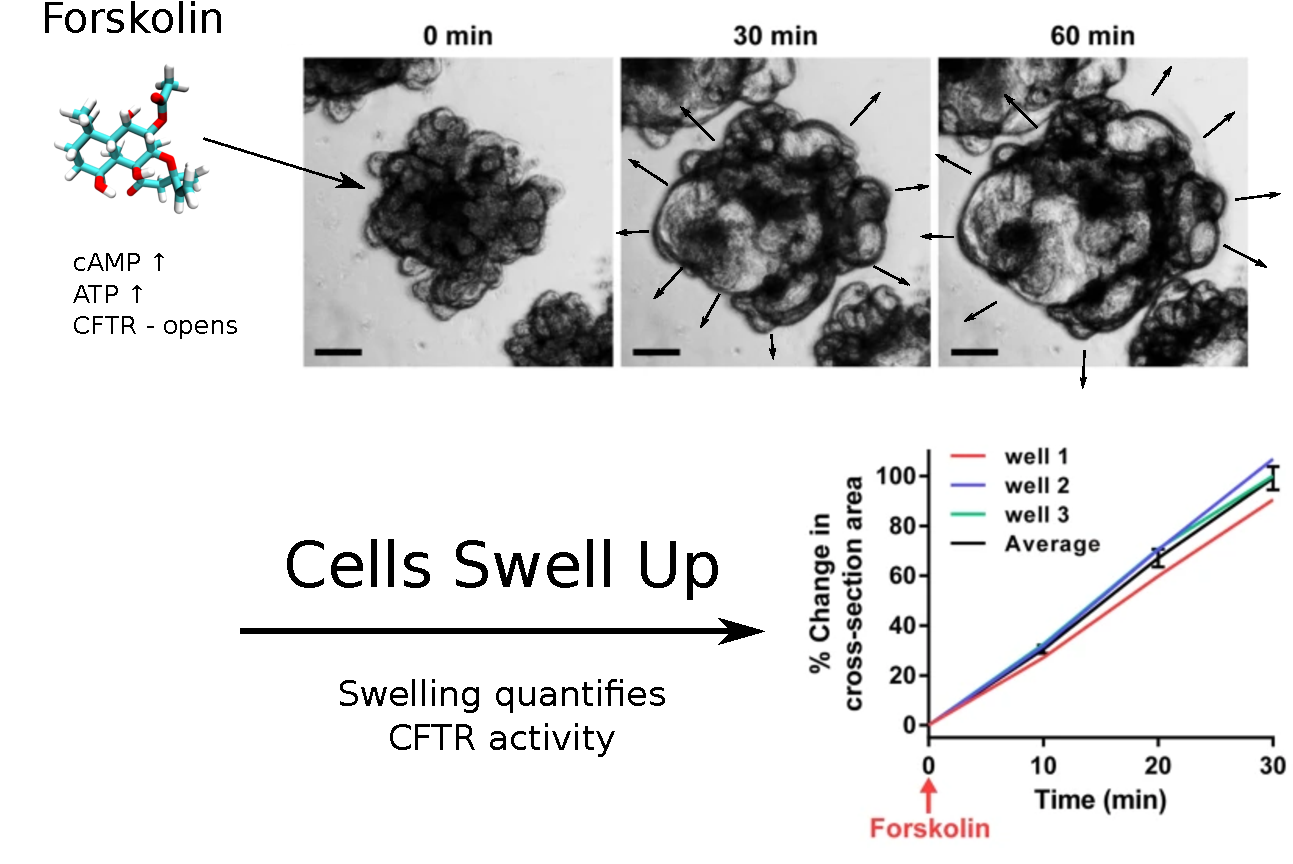
\includegraphics[width=1\textwidth]{figures/FIS_demo.pdf}
	\end{center}
	\captionsetup{singlelinecheck = false, justification=raggedright}
	\caption[Forskolin Induced Swelling] {\textbf{Forskolin Induced Swelling}}{Upon exposure to Forskolin, epithelial cells begin to produce cAMP. This causes an increase in intracellular ATP which will open CFTR channels. The influx of water into the cell causes them to swell. The amount of swelling can be used to quantify the amount of properly functioning CFTR in the cell.} 
\end{figure}
Forskolin Induced Swelling (FIS) assays can be used used to easily characterise the amount of functioning CFTR in a patients cells \cite{dekkers2013}. When epithelial cells are exposed to a chemical known as forskolin they begin to rapidly produce cyclic AMP (cAMP, a precursor to ATP in a cell) \cite{bonora2012}. The presence of ATP activates the CFTR ion channels, causing the cells themselves to swell due to the intake of moisture. When performed under a micropsope with patient derived orgnaoids, this swelling allows cell biologists to easily quantify the activity of CFTR within a cell in a variety of conditions, such as the presence of drugs.

Hence, by comparing the amount of swelling swelling of organoids in the presence or absence of modulators, we can quantitatively assess the response of a patient's cells to modulator therapy (Figure \ref{FIS_figure}). 

\subsection{Electrophysiology Directly Measures CFTR Gating and Conduction}
The measurement of electrical activity in biological systems is known as electrophysiology. This field has been an important way for us to develop models for the activity of ion channels and the cells which host them \cite{aidley1996}. Since CFTR is an ion channel, measuring its electrical activity is a direct way to assess its function and dynamics, leading to a molecular understanding of the nature of disease. A comprehensive review of techniques, specifically developed to investigate CFTR can be found in \cite{cui2021}.

In order to study the action of a single ion channel one needs to employ an experimental technique known as patch clamp electrophysiology \cite{hille2001}. Studies using this technique were vital for the conclusions of chapters \ref{chap:R352Q} and \ref{chap:opening}. For a comprehensive view of modelling from patch clamp derived data see \cite{cai2011}. On the other hand, to assess the competency of a whole membrane or tissue, to understand the effect of a CFTR on a whole organ, one instead uses what is known as an Ussing chamber \cite{hoenig2014}. This was a technique used extensively by collaborators of our MD modelling, where epithelia grown from a patient's own cells were placed in an Ussing chamber so their competency to diffuse chloride could be measured.

\subsubsection{Patch Clamp Electrophysiology}
\begin{figure}
	\begin{center}
	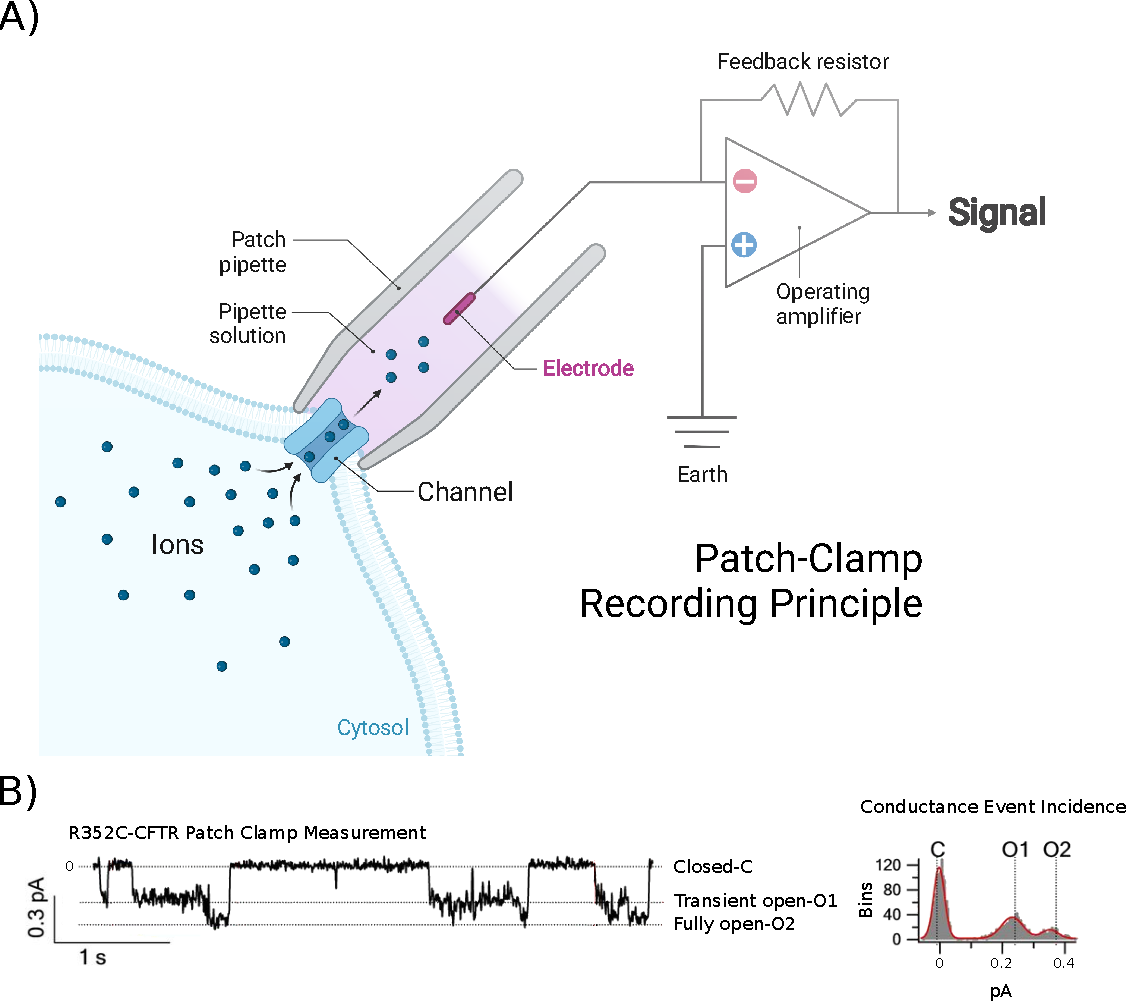
\includegraphics[width=0.8\textwidth]{figures/R352C_ephys_measurement_figure.pdf}
	\end{center}
	\captionsetup{singlelinecheck = false, justification=raggedright}
	\caption[Patch Clamp Apparatus] {\textbf{Patch Clamp Apparatus}}{A) In patch clamp electrophysiology, a micropipette is placed against the membrane to create a tight seal \cite{patch_clamp_recording_principal_figure}. B) The current trace from the measurement of a mutant CFTR channel. The R352C mutant was chosen for visualisation as it shows a clearly shows two open states: a transient state with lower conductance, known as the O1 state and a fully open state known as the O2 state \cite{jih2012}. The accidental discovery of this mutant has been used extensively in studying the gating cycle of CFTR, giving an interesting example an example of how useful electrophysiology can be for molecular biophysics. Source data from \cite{jih2012}. Note that this mutant has roughly half the conductance of WT-CFTR.} 
	\label{patch_clamp}
\end{figure}

Patch Clamp Electrophysiology has been critical to the development of molecular biophysics in ion channels. Through the use of a micropipette filled with electrolyte solution, we can measure the activity of a single ion channel. As shown in figure \ref{patch_clamp}, the tip of a micropipette is placed directly on a cell membrane in order to measure the current flowing through a single ion channel. A single ion channel exhibits a current on the order of 1 picoAmp (for reference, CFTR exhibits 0.7pA at a bias voltage of 100 mV), so the formation of a tight seal with the membrane is critical to filter out noise. To tighten this seal, a small amount of suction is usually applied to the membrane through the pipette \cite{aidley1996}.

In the inside-out variant of this technique, the ion channel along with a small patch of membrane is excised, exposing the system to the surrounding bath. This means that the response of the ion channel to different chemical conditions can be tested by changing the composition of the bath. Patch clamp electrophysiology experiments are not presented in this thesis but they considered closely when writing chapter \ref{chap:opening}  so an outline of them has been given here.

\subsubsection{Ussing Chambers}
An Ussing chamber is a versatile apparatus which allows the measurement of current across an epithelial membrane. In chapters \ref{chap:I37R}, \ref{chap:R352Q} and \ref{chap:S945L}, they were used extensively. Here, a mono-layer was derived from an organoid and used as a patch in the Ussing chamber. By blocking other ion channels such as ENaC during measurements, a clear picture of CFTR function can be measured in order to create an understanding of the nature of disease in each patient. The monolayer could also be exposed to different regimens of modulators in order to assess the ability of those modulators to rescue the function of the organoid. The higher the current, the more CFTR proteins were functioning and the better the rescue of the mutation.

In Ussing chamber measurements, current is usually expressed as amps per unit area, which normalises the measurement to the size of the patch. It is also important that the patch of epithelial membrane is continuous, as holes would allow current to pass unrestricted give errantly high readings. This highlights how great care must be taken when growing organoids. 


\begin{figure}
	\label{ussing_chamber}
	\begin{center}
	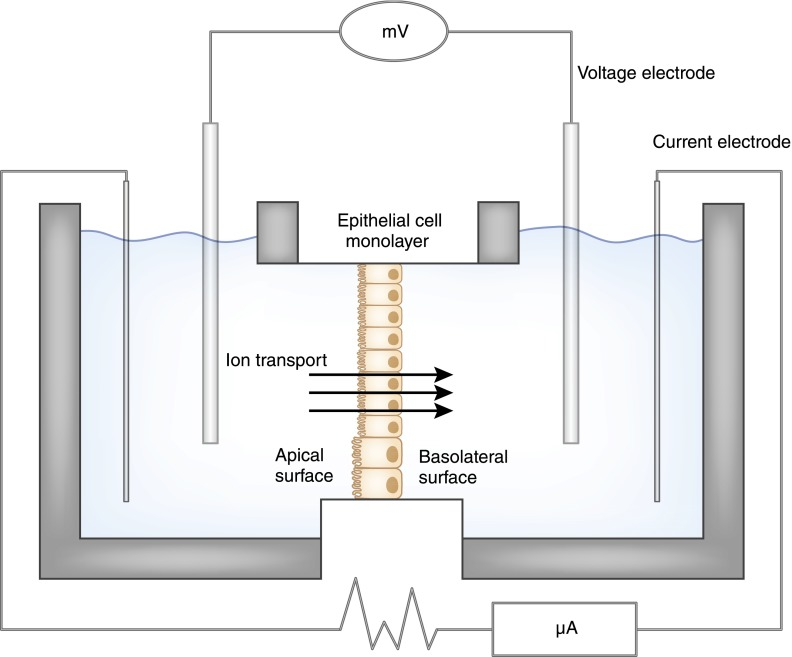
\includegraphics[width=0.4\textwidth]{figures/ussing_chamber.jpg}
	\end{center}
	\captionsetup{singlelinecheck = false, justification=raggedright}
	\caption[Ussing Chamber Setup] {\textbf{Ussing Chamber Setup}}{Ussing chambers can be used to characterise the function of an epithelial monolayer. The membrane can be exposed to different cellular conditions and its conductance can be measured under these conditions to test different drugs. For our purposes, an Ussing chamber may be used to measure the ion transport of an epithelium grown from a patient derived organoid. Source \cite{hoenig2014}} 
\end{figure}


\subsection{Western Blotting Assesses CFTR Trafficking}
\begin{figure}
	\begin{center}
	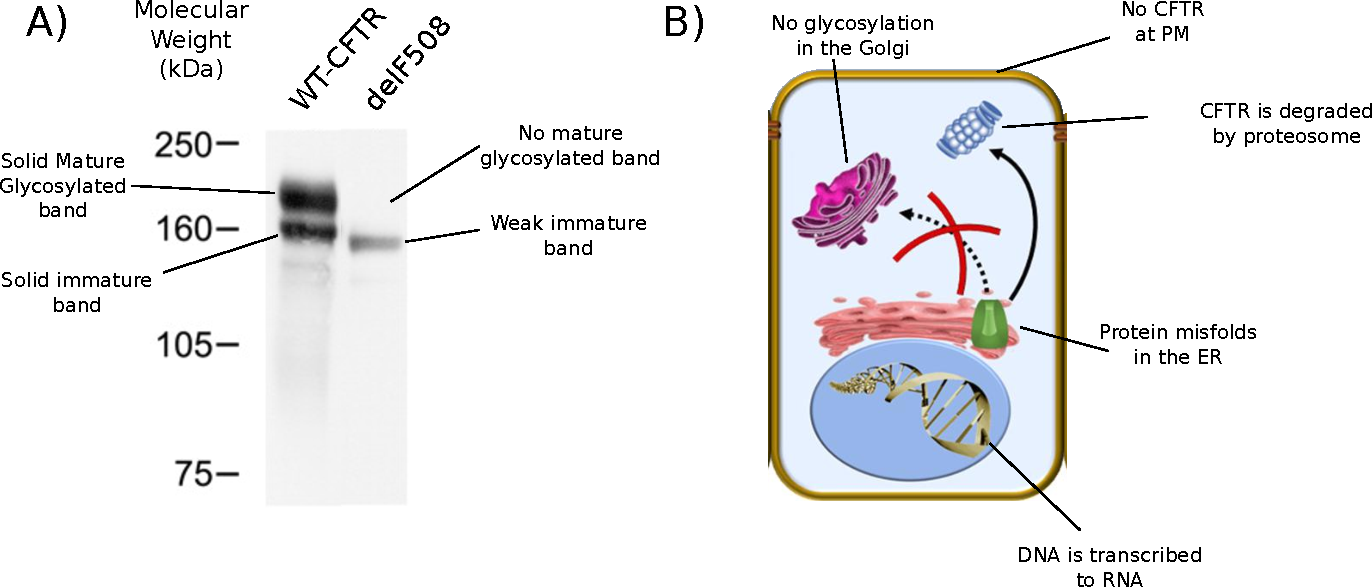
\includegraphics[width=1\textwidth]{figures/western_blot_explanation.pdf}
	\end{center}
	\captionsetup{singlelinecheck = false, justification=raggedright}
	\caption[Western Blot Explanation] {\textbf{Western Blot Explanation}}{A) Output of a western blot experiment. WT-CFTR has much more abundant protein than $\Delta$F508 \cite{chang2008}. B) The cell biology behind why the $\Delta$F508 mutation is pathogenic. When WT-CFTR folds correctly in the Endoplasmic reticulum it is trafficked into the Golgi where it is glycosylated, before it is then implanted into the cell membrane. In the case of $\Delta$F508, the protein misfolds as it is synthesised, so instead of being trafficked as normally it is prematurely degraded by the proteosome \cite{lopes-pacheco2016a, lewis2005}.} 
	\label{western_blot}
\end{figure}
The above methods focus on measuring the electrical activity of the ion channels once they are at the cell membrane, they will only detect functional channels. In order to test the presence of ion channels within the epithelium, functional or otherwise, a technique called western blotting is employed (Figure \ref{western_blot}).

A simplified explanation of the most common technique is given below but there are many variations
\begin{enumerate}
	\item The proteins in the sample of cells are denatured, sometimes by boiling. This makes them unfold and stretch out into long peptides. 
	\item The proteins in the sample are injected into an agar gel.
	\item The gel is immersed in a buffer solution and a voltage is applied to it in a process known as electrophoresis. This causes proteins to migrate through the gel according to their charge to mass ratio. The heavier the protein, the less it will move. 
	\item The presence of proteins is visualised through immunostaining. First, the gel is washed with a primary antibody. This antibody is specific protein we wish to detect (in our case, CFTR). 
	\item The excess primary antibody is washed off the gel, but some of the antibodies will stay bound to the proteins we are interested in. 
	\item A secondary antibody is washed over the gel. This is engineered to bind to the primary antibody. What is important about the secondary antibody is that it is attached to a special enzyme tag, which we can visualise.  
	\item The excess secondary antibody is washed off the gel, but but some of the secondary antibodies will remain bound to the primary antibody.
	\item The tag on the secondary antibody is visualised through the use of chemiluminesence. The tag is typically an enzyme, which emits light when it breaks down a substrate. Hence, for the visualisation step, a photographic film is placed over the gel and it is washed a final time, in the substrate of the enzyme which the secondary antibody is attached to. This produces bands in the photographic film, the darker the band is at position, and the more of the target is present there.
\end{enumerate}
By washing the gel in different primary antibodies, we can detect multiple proteins in one experiment. This is often used to normalise the quantity protein measured between samples. Hence, one will often see structural proteins such as tubulin or actin in figures showing the results from a western blot. These are used as controls and should not change due to between experiments. Western blotting is thus a simple, widely used technique to quantify the amount of specific proteins in the cell. 

\section{Conclusion}

Note throughout the chapters ahead how we have relied on results from careful biochemical and biophysical literature which elucidated the molecular details of the function and misfunction of CFTR. Close reading of these studies was necessary in order to form hypothesise about the function of CFTR which we could test \textit {in silico}. 

In biophysics, it is only through the collection of \textit{in vitro} data through which we can formulate our theoretical models. So we are grateful for the painstaking work of Paul Linsdell, Christine E. Bear, Robert Ford, Laszslo Csandy, Tzyh-Chang Hwang, Naels Mccarty, Isabelle Callebaut, John Paul Mornon, David Gadsby, Jue Chen, Ina Urbatsch, John Hunt, Julie D. Foreman Kay and all the members of their laboratories for their detailed studies of the CFTR protein. This is not to discount the work which went into the identification of the CFTR gene \cite{riordan1989}, nor the outstanding work of the clinicians and physicians who work with patients to understand more about the nature of the disease \cite{roberts1957}.  

As was mentioned in the \href{Foreword} {\ref{chap:foreword}}, experts from many fields must all work together to understand the whole organism and thanks to decades of work by hundreds of people we have a host of molecular details which we can combine in order to understand the function and misfunction of CFTR. In the next 4 chapters we will combine some of these details, alongside our own findings from organoid studies and simulations to make our own contribution to the molecular understanding of Cystic Fibrosis as a disease. This literature will again be used for our conclusion in chapter \ref{chap:conclusion} to push for certain questions to be answered in molecular CF research.

CFTR is just one protein. It's a complicated one to be sure but it's far from the most complicated in a mammalian cell \cite{saotome2018, zalk2015, chen2018a}. I hope that this chapter has given an appreciation of the level of detail that exists in biological systems. Remember that there are an estimated 42 million individual protein molecules in each cell, in more than 20 thousand variates \cite{ho2018, salzberg2018}. The decades of insight into CFTR was motivated by the terrible disease it is responsible for, but this also gives us the opportunity to demonstrate the power and insight gained from a molecular understanding of disease. The next 4 chapters will be examples how to combine the simulations we looked at in chapter \ref{chap:methods} with insights from patient specific assays, to understand more about CF pathogenesis. These results will be tied together in chapter \ref{chap:conclusion} to help us understand \textit{how} drugs are rescuing CFTR function and the direction this conclusion would suggest for research into treating the root cause of CF.

